\documentclass[a4paper]{report}
%----------japanese text command----------%
\newcommand{\jp}[1]{\begin{CJK}{UTF8}{min}#1\end{CJK}} 

%----------items----------%
\newcommand{\potion}[1][]{Potion #1(\jp{ポーション})}
\newcommand{\hiPotion}[1][]{HiPotion #1(\jp{ハイポーション})}
\newcommand{\phoenixDown}[1][]{Phoenix Down #1(\jp{フェニックスの尾})}
\newcommand{\revivify}[1][]{Revivify #1(\jp{せいすい})}
\newcommand{\maidensKiss}[1][]{Maiden's Kiss #1(\jp{おとめのキッス})}
\newcommand{\eyedrop}[1][]{Eyedrop #1(\jp{めぐすり})}
\newcommand{\antidote}[1][]{Antidote #1(\jp{どくけし})}
\newcommand{\tent}[1][]{Tent #1(\jp{テント})}
\newcommand{\flameScroll}[1][]{Flame Scroll #1(\jp{かとんのじゅつ})}
\newcommand{\elixir}[1][]{Elixir #1(\jp{エリクサー})}
\newcommand{\waterScroll}[1][]{Water Scroll #1(\jp{すいとんのじゅつ})}
\newcommand{\thunderScroll}[1][]{Thunder Scroll #1(\jp{らいじんのじゅつ})}
\newcommand{\cottage}[1][]{Cottage #1(\jp{コテージ})}
\newcommand{\ether}[1][]{Ether #1(\jp{エーテル})}
\newcommand{\speedDrink}[1][]{Speed Drink #1(\jp{スピードドリンク})}
\newcommand{\heroDrink}[1][]{Hero Drink #1(\jp{えいゆうのくすり})}
\newcommand{\turtleShell}[1][]{Turtle Shell #1(\jp{かめのこうら})}
\newcommand{\dragonFang}[1][]{Dragon Fang #1(\jp{りゅうのきぼ})}

%----------spells----------%
\newcommand{\life}[1][]{Life #1(\jp{レイズ})}
\newcommand{\fire}[1][]{Fire #1(\jp{ファイア})}
\newcommand{\bolt}[1][]{Bolt #1(\jp{サンダー})}
\newcommand{\cure}[1][]{Cure #1(\jp{ケアル})}
\newcommand{\goblinPunch}[1][]{Goblin Punch #1(\jp{ゴブリンパンチ})}
\newcommand{\exit}[1][]{Exit #1(\jp{テレポ})}
\newcommand{\reset}[1][]{Reset #1(\jp{リターン})}
\newcommand{\breakSpell}[1][]{Break #1(\jp{ブレイク})} 
\newcommand{\ltwoOld}[1][]{L.2 Old #1(\jp{レベル2オールド})} 
\newcommand{\lfiveDeath}[1][]{L.5 Death #1(\jp{レベル5デス})} 
\newcommand{\size}[1][]{Size #1(\jp{ミニマム})}
\newcommand{\float}[1][]{Float #1(\jp{レビテト})}
\newcommand{\reflect}[1][]{Reflect #1(\jp{リフレク})}
\newcommand{\haste}[1][]{ヘイスト #1(\jp{リフレク})}

%----------abilities----------%
\newcommand{\gilToss}[1][]{Gil Toss #1(\jp{ぜになげ})}
\newcommand{\cover}[1][]{Cover #1(\jp{かぼう})}
\newcommand{\combine}[1][]{Combine #1(\jp{ちょうごう})}
\newcommand{\black}[1][]{Black #1(\jp{くろまほう})} 
\newcommand{\blue}[1][]{Blue #1(\jp{あおまほう})} 
\newcommand{\magicSword}[1][]{Magic Sword #1(\jp{まほうけん})} 
\newcommand{\kick}[1][]{Kick #1(\jp{けり})} 
\newcommand{\guard}[1][]{Guard #1(\jp{まもる})}
\newcommand{\steal}[1][]{Steal #1(\jp{盗む})}
\newcommand{\throw}[1][]{Throw #1(\jp{なげる})}
\newcommand{\catch}[1][]{Catch #1(\jp{とらえる})}
\newcommand{\observe}[1][]{Observe #1(\jp{しらべる})}
\newcommand{\release}[1][]{Release #1(\jp{はなつ})}
\newcommand{\white}[1][]{White #1(\jp{しろまほう})} 
\newcommand{\escape}[1][]{Escape #1(\jp{とんずら})} 
\newcommand{\tame}[1][]{Tame #1(\jp{なだめる})} 
\newcommand{\gaia}[1][]{Gaia #1(\jp{ちけい})} 
\newcommand{\hide}[1][]{Hide #1(\jp{かくねる})} 
\newcommand{\drink}[1][]{Drink #1(\jp{のむ})} 
\newcommand{\dash}[1][]{Dash #1(\jp{ダッシュ})} 
\newcommand{\learning}[1][]{Learning #1(\jp{ラーニング})} 
\newcommand{\control}[1][]{Control #1(\jp{あやつる})} 
\newcommand{\dimenAbility}[1][]{Dimen #1(\jp{じくう})} 
\newcommand{\showAbility}[1][]{Show #1(\jp{あらねれる})} 

%----------weapons----------%
\newcommand{\broadsword}[1][]{Broadsword #1(\jp{ブロードソード})}
\newcommand{\knife}[1][]{Knife #1(\jp{ナイフ})}
\newcommand{\daggerWeapon}[1][]{Dagger #1(\jp{ダガー})}
\newcommand{\iceRod}[1][]{Ice Rod #1(\jp{こおりのロッド})}
\newcommand{\mythrilKnife}[1][]{Mythril Knife #1(\jp{ミスリルナイフ})}
\newcommand{\fireRod}[1][]{Fire Rod #1(\jp{ほのおのロッド})}
\newcommand{\thunderRod}[1][]{Thunder Rod #1(\jp{いかづのロッド})}
\newcommand{\kunai}[1][]{Kunai #1(\jp{くない})}
\newcommand{\shuriken}[1][]{Shuriken #1(\jp{しゅりけん})}
\newcommand{\ancientSword}[1][]{Ancient Sword #1(\jp{こだいのつるぎ})}
\newcommand{\dancingDagger}[1][]{Dancing Dagger #1(\jp{ダンシングダガー})}
\newcommand{\airBlade}[1][]{Air Blade #1(\jp{かぜきりのやいば})}

%----------armor----------%
\newcommand{\crystalShield}[1][]{Crystal Shield #1(\jp{クリスタルのたて})}
\newcommand{\silkRobe}[1][]{Silk Robe #1(\jp{シルクのローブ})}
\newcommand{\stealthRobe}[1][]{Stealth Robe #1(\jp{しのびのころも})}
\newcommand{\goldArmor}[1][]{Gold Armor #1(\jp{ゴールドアーマー})}
\newcommand{\iceBow}[1][]{Ice Bow #1(\jp{こおりのゅみや})}
\newcommand{\powerWrist}[1][]{Power Wrist #1(\jp{パワーリスト})}
\newcommand{\greenBeret}[1][]{Green Beret #1(\jp{グリーンベレー})}
\newcommand{\goldShield}[1][]{Gold Shield #1(\jp{ゴールドシールド})}
\newcommand{\boneMail}[1][]{Bone Mail #1(\jp{ボーンメイル})}
\newcommand{\iceShield}[1][]{Ice Shield #1(\jp{アイスシールド})}
\newcommand{\ribbon}[1][]{Ribbon #1(\jp{リボン})}

%----------accessories----------%
\newcommand{\runningShoes}[1][]{Running Shoes #1(\jp{エルメスのくつ})}
 
%----------misc----------%
\newcommand{\activeOption}[1][]{Active #1(\jp{アクティヴ})}
\newcommand{\shortOption}[1][]{Short #1(\jp{たんしゆく})}
\newcommand{\memoryOption}[1][]{Memory #1(\jp{きおく})}
\newcommand{\emptyOption}[1][]{Empty #1(\jp{すべてはずす})}
\usepackage[group-separator={,},group-minimum-digits={3}]{siunitx}
\usepackage[utf8]{inputenc}
\usepackage[dvipsnames]{xcolor}
\usepackage{tcolorbox}
\usepackage[margin=0.2in, paperwidth=12in]{geometry}
\usepackage{setspace}
\usepackage{hyperref}
\usepackage{titlepic}
\usepackage{CJKutf8}
\usepackage{soulutf8}
\usepackage{varwidth}
\usepackage{tocloft}
\usepackage{paracol} 

%----------page setup----------%
\definecolor{pageColor}{RGB}{240, 240, 240}
\pagecolor{pageColor}
\setlength{\columnsep}{.5cm}
\hfuzz=49pt 

%----------chapter setup----------%
\makeatletter
\def\@makechapterhead#1{%
  {\parindent \z@ \normalfont
    \ifnum \c@secnumdepth >\m@ne
        \huge\bfseries #1
        \par\nobreak
        \rule{\columnwidth}{.1pt}%
    \fi
    \interlinepenalty\@M
  }}
\makeatother

%----------hyperlinks----------%
\hypersetup{
    colorlinks,
    citecolor=black,
    filecolor=black,
    linkcolor=black,
    urlcolor=black
}

%----------misc setup----------%
\usepackage{enumitem}
\setitemize{noitemsep,topsep=0pt,parsep=0pt,partopsep=0pt}
\usepackage{graphicx}

\pagenumbering{gobble}
\setlength{\columnsep}{1.5cm}
\setlength{\columnseprule}{0.2pt}

\makeatletter
\patchcmd{\chapter}{\if@openright\cleardoublepage\else\clearpage\fi}{}{}{}
\makeatother

\DeclareUnicodeCharacter{2194}{\ensuremath{\leftrightarrow}}

%---------toc--------------%
\setlength{\cftbeforetoctitleskip}{-3.5mm}
\renewcommand{\cfttoctitlefont}{\Huge\bfseries}
\renewcommand{\cftaftertoctitle}{\par\nobreak\rule{\columnwidth}{.1pt}}

%----------style overrides----------%
\renewcommand{\theenumi}{\textbf{\arabic{enumi}}}
\renewcommand{\labelitemi}{$\bullet$}
\renewcommand{\labelitemii}{$\circ$}
\renewcommand{\labelitemiii}{$\ast$}
\renewcommand{\labelitemiv}{$-$}
\renewcommand{\familydefault}{\sfdefault}

%----------convenience commands----------%
\newcommand{\insertStep}[1]{\includegraphics[scale=0.598]{#1}}
\newcommand{\insertBattleMenu}[1]{\includegraphics[scale=1.655]{#1}}
\newcommand{\insertMisc}[1]{\includegraphics[scale=0.469]{#1}}
\newcommand{\insertScreenshot}[1]{\includegraphics[scale=0.621]{#1}}
\newcommand{\varwb}{\begin{varwidth}{\textwidth}}
\newcommand{\varwe}{\end{varwidth}}
\newcommand{\resume}{\vspace{-1pc}}
\newcommand{\switchcolumnTwice}[1][]{\switchcolumn\switchcolumn#1}

%----------arrows----------%
\newcommand{\pointUp}{\textbf{↑}}
\newcommand{\pointDown}{\textbf{↓}}
\newcommand{\pointLeft}{\textbf{←}}
\newcommand{\pointRight}{\textbf{→}}
\newcommand{\switch}{\textbf{↔ }}
\newcommand{\then}{\textbf{→ }}

%----------base colors----------%
\definecolor{red}{RGB}{234, 52, 35}
\definecolor{blue}{RGB}{47, 152, 222}
\definecolor{purple}{RGB}{139, 70, 229}
\definecolor{pink}{RGB}{235, 18, 127}
\definecolor{orange}{RGB}{245, 122, 0}
\definecolor{green}{RGB}{0, 181, 133}
\definecolor{yellow}{RGB}{253, 255, 84}

%----------colorbox colors----------%
\definecolor{menu}{RGB}{72, 188, 72}
\colorlet{menuHl}{menu!55}
\definecolor{shop}{RGB}{228, 162, 9}
\colorlet{shopHl}{shop!55}
\colorlet{shopNoteHl}{blue!45}
\definecolor{boss}{RGB}{229, 51, 51}
\colorlet{bossHl}{boss!55}
\colorlet{bossNoteHl}{orange!50}
\definecolor{encounter}{RGB}{223, 113, 168}
\colorlet{encounterHl}{encounter!55}
\colorlet{encounterNoteHl}{purple!45}
\definecolor{steproute}{RGB}{79, 173, 235}
\colorlet{stepHl}{blue!45}
\definecolor{misc}{RGB}{9, 191, 198}
\colorlet{miscHl}{misc!55}

%----------additional colors----------%
\colorlet{dialog}{orange}
\colorlet{pickup}{purple}
\colorlet{optimize}{pink}
\colorlet{ability}{orange}
\colorlet{equip}{purple}
\colorlet{battleGroup}{pink}
\colorlet{ally}{blue}
\colorlet{enemy}{red}
\colorlet{unequip}{red}
\colorlet{leftCommand}{purple}
\colorlet{rightCommand}{green}

%----------highlights----------%
\newcommand{\menuHl}[1]{\sethlcolor{menuHl}\textbf{\hl{#1}}}
\newcommand{\shopHl}[1]{\sethlcolor{shopHl}\textbf{\hl{#1}}}
\newcommand{\shopNote}[1]{\sethlcolor{shopNoteHl}\textbf{\hl{#1}}}
\newcommand{\encounterHl}[1]{\sethlcolor{encounterHl}\textbf{\hl{#1}}}
\newcommand{\encounterNote}[1]{\sethlcolor{encounterNoteHl}\textbf{\hl{#1}}}
\newcommand{\encounterMenu}[1]{\sethlcolor{encounterNoteHl}\hl{#1}}
\newcommand{\bossHl}[1]{\sethlcolor{bossHl}\textbf{\hl{#1}}}
\newcommand{\bossNote}[1]{\sethlcolor{bossNoteHl}\textbf{\hl{#1}}}
\newcommand{\bossMenu}[1]{\sethlcolor{bossNoteHl}\hl{#1}}
\newcommand{\miscHl}[1]{\sethlcolor{miscHl}\textbf{\hl{#1}}}
\newcommand{\stepHl}[1]{\sethlcolor{stepHl}\textbf{\hl{#1}}}

%----------color boxes----------%
\newtcolorbox{menu}[2][]{colframe=menu!55, colback=menu!20, coltitle=menu!20!black, title={\textbf{#2}}, #1}
\newtcolorbox{encounter}[2][]{colframe=encounter!55, colback=encounter!20, coltitle=encounter!20!black, title={\textbf{#2}}, #1}
\newtcolorbox{shop}[2][]{colframe=shop!55, colback=shop!20, coltitle=shop!20!black, title={\textbf{#2}}, #1}
\newtcolorbox{boss}[2][]{colframe=boss!55, colback=boss!20, coltitle=boss!20!black, title={\textbf{#2}}, #1}
\newtcolorbox{steproute}[2][]{colframe=steproute!55, colback=steproute!20, coltitle=steproute!20!black, title={\textbf{#2}}, #1}
\newtcolorbox{misc}[2][]{colframe=misc!55, colback=misc!20, coltitle=misc!20!black, title={\textbf{#2}}, #1}

%----------color box item options----------%
\newenvironment{configMenu}{\begin{itemize}\item\ul{Config}\begin{itemize}}{\end{itemize}\end{itemize}}
\newenvironment{jobMenu}{\begin{itemize}\item\ul{Job}\begin{itemize}}{\end{itemize}\end{itemize}}
\newenvironment{magicMenu}{\begin{itemize}\item\ul{Magic}\begin{itemize}}{\end{itemize}\end{itemize}}
\newenvironment{itemMenu}{\begin{itemize}\item\ul{Item}\begin{itemize}}{\end{itemize}\end{itemize}}
\newenvironment{equipMenu}{\begin{itemize}\item\ul{Equip}\begin{itemize}}{\end{itemize}\end{itemize}}
\newenvironment{abilityMenu}{\begin{itemize}\item\ul{Ability}\begin{itemize}}{\end{itemize}\end{itemize}}

\newenvironment{rowMenu}{\begin{itemize}\item\ul{Row}\begin{itemize}}{\end{itemize}\end{itemize}}
\newenvironment{round}[1]{\begin{itemize}\item\ul{Round #1}\begin{itemize}}{\end{itemize}\end{itemize}}
\newenvironment{bossPart}[1]{\begin{itemize}\item\ul{#1}\begin{itemize}}{\end{itemize}\end{itemize}}
\newenvironment{buy}[1][]{\begin{itemize}\item\ul{Buy#1}\begin{itemize}}{\end{itemize}\end{itemize}}
\newenvironment{sell}{\begin{itemize}\item\ul{Sell}\begin{itemize}}{\end{itemize}\end{itemize}}
\newenvironment{notes}{\begin{itemize}}{\end{itemize}}

%----------party members----------%
\newcommand{\bartz}[1][]{\item #1 \textbf{Bartz: }}
\newcommand{\lenna}[1][]{\item #1 \textbf{Lenna: }}
\newcommand{\faris}[1][]{\item #1 \textbf{Faris: }}
\newcommand{\galuf}[1][]{\item #1 \textbf{Galuf: }}
\newcommand{\cara}[1][]{\item #1 \textbf{Cara: }}
\newcommand{\bartzFaris}[1][]{\item #1 \textbf{Bartz/Faris: }}
\newcommand{\galufLenna}[1][]{\item #1 \textbf{Galuf/Lenna: }}
\newcommand{\lennaFaris}[1][]{\item #1 \textbf{Lenna/Faris: }}
\newcommand{\caraFarisBartz}[1][]{\item #1 \textbf{Cara/Faris/Bartz: }}
\newcommand{\everyone}[1][]{\item #1 \textbf{Everyone: }}
\newcommand{\everyoneElse}[1][]{\item #1 \textbf{Everyone Else: }}
\newcommand{\anyone}[1][]{\item #1 \textbf{Anyone: }}
\newcommand{\ninjas}[1][]{\item #1 \textbf{Ninjas: }}
\newcommand{\swap}{\item \textbf{Swap: }}

%----------commands----------%
\newcommand{\pickup}[1]{\textbf{\textcolor{pickup}{#1}}}
\newcommand{\dialog}[1]{\textbf{\textcolor{dialog}{(#1)}}}

\newcommand{\battleGroup}[1]{\textbf{\textcolor{battleGroup}{#1}}}
\newcommand{\enemy}[1]{\textbf{\textcolor{enemy}{#1}}}
\newcommand{\ally}[1]{\textbf{\textcolor{ally}{#1}}}
\newcommand{\leftCommand}[1]{\textbf{\textcolor{leftCommand}{#1}}}
\newcommand{\rightCommand}[1]{\textbf{\textcolor{rightCommand}{#1}}}

\newcommand{\potionMenu}[1][]{\item \textbf{\potion: }}
\newcommand{\hiPotionMenu}[1][]{\item \textbf{\hiPotion: }}
\newcommand{\phoenixDownMenu}[1][]{\item \textbf{\phoenixDown: }}
\newcommand{\cureMenu}[1][]{\item \textbf{\cure: }}
\newcommand{\antidoteMenu}[1][]{\item \textbf{\antidote: }}
\newcommand{\maidensKissMenu}[1][]{\item \textbf{\maidensKiss: }}
\newcommand{\elixirMenu}[1][]{\item \textbf{\elixir: }}

\newcommand{\ability}[1]{\textbf{\textcolor{ability}{#1}}}
\newcommand{\unequip}[1]{\textbf{\textcolor{unequip}{#1}}}
\newcommand{\optimize}{\textbf{\textcolor{optimize}{Optimize}}}
\newcommand{\equip}[1]{\textbf{\textcolor{equip}{#1}}}

%----------title----------%
\title{\textbf{\Huge{Final Fantasy V \\ 
  Any\% Glitchless BS1A}}}
\author{\LARGE{by Tojju}}
\date{\vspace{-5ex}}
\titlepic{
\includegraphics[scale=0.4]{../Graphics/Misc/1. FFV Logo.png}}
\begin{document}
\singlespacing
\maketitle
\tableofcontents
\addtocontents{toc}{\vspace{-1cm}}

%----------acknowledgements----------%
\section*{Acknowledgements}
Giru (\jp{ギル}), Zinfogel, MrTyton

\setlength{\columnseprule}{0.2pt}
\chapter{World One}

\vspace{\baselineskip}

\begin{paracol}{2}

\begin{menu}{After Dismounting Boko}
	\varwb
	\begin{configMenu}
		\item \menuHl{(1)} \textbf{Bat.Mode:} \activeOption
		\item \menuHl{(2)} \textbf{Bat.Speed:} 1
		\item \menuHl{(3)} \textbf{Msg.Speed:} 1
		\item \menuHl{(4)} \textbf{Cmd.Set:} \shortOption
		\item \menuHl{(7)} \textbf{Cursor:} \memoryOption
		\item \menuHl{(8)} \textbf{Reequip:} \emptyOption
	\end{configMenu}
	\varwe
\end{menu}

\begin{encounter}{Goblin x2}
	\varwb
	\begin{round}{1 (Onward)}
		\bartz Fight
	\end{round}
	\varwe
\end{encounter}

\begin{enumerate}
	\item Name Bartz  “\jp{\textbf{あ}}”: (\pointDown)(\textbf{A})(\pointUp)(\textbf{2}\pointRight)(\textbf{A})
\end{enumerate}

\begin{encounter}{Goblin x2 (x2)}
	\varwb
	\begin{round}{1 (Onward)}
		\bartz Fight
	\end{round}
	\varwe
\end{encounter}

\begin{enumerate}[resume]
	\item Enter the cave
\end{enumerate}

\resume
\begin{enumerate}[resume]
	\item Deny the pirate when he offers to help \dialog{2nd}
\end{enumerate}

\end{paracol}
\chapter{Wind Shrine}

\vspace{\baselineskip}

\begin{paracol}{2}

\begin{encounter}{White Snake (5 EXP)}
	\varwb
	\begin{notes}
		\item \encounterHl{Don't flee buffer}
	\end{notes}
	\begin{round}{1}
		\faris Fight
	\end{round}
	\varwe
\end{encounter}

\switchcolumn
\begin{steproute}{Wind Shrine Encounter}
	\begin{itemize}[leftmargin=*]
		\item[] Any single enemy encounter will suffice
	\end{itemize}
\end{steproute}

\switchcolumn
\begin{enumerate}
	\item Grab the \pickup{Broadsword} next to the hidden passage
\end{enumerate}

\begin{boss}{Wing Raptor}
	\varwb
	\begin{round}{1}
		\everyone Fight
		\galuf Item \then \battleGroup{Equip \broadsword} \then Fight
	\end{round}
	\begin{round}{2}
		\everyone Fight
	\end{round}
	\varwe
\end{boss}

\begin{menu}{After Getting the First Set of Jobs}
	\varwb
	\begin{jobMenu}
		\faris Black Mage \textbf{(3\pointLeft)}
		\bartz Thief \textbf{(2\pointRight)} \optimize
		\lenna Blue Mage \textbf{(2\pointLeft)} \optimize
		\galuf Blue Mage \textbf{(2\pointLeft)} \optimize
	\end{jobMenu}
	\varwe
\end{menu}

\begin{enumerate}[resume]
	\item Exit via the newly opened passage
	\item Deny the chocobo when he offers to help \dialog{2nd}
\end{enumerate}

\end{paracol}


\chapter{Tule}

\vspace{\baselineskip}

\begin{paracol}{2}

\begin{enumerate}
    \item Head to the Beginner's House
    \item Grab the following chests: \pickup{Tent, Potion, Ether, Phoenix Down, and 100 Gil} 
\end{enumerate}

\switchcolumn
\begin{misc}{Beginner's House Treasure}
    \insertMisc{../Graphics/Misc/2. Beginners House.png}
\end{misc}

\switchcolumn
\resume
\begin{enumerate}[resume]
    \item Head upstairs and open the monster chest
\end{enumerate}

\begin{encounter}{Goblin}
    \varwb
    \begin{round}{1 (Onwards)}
        \bartz Fight \pointRight \space \ally{Bartz}
        \lenna Fight \pointRight \space \ally{Bartz}
        \item \encounterMenu{\textbf{Blank:} slot 1 + 3}
        \vspace{1mm}
        \item[] \insertBattleMenu{../Graphics/Battle/1. Goblin Punch Menu.png}
        \item Wait until he uses Goblin Punch
        \galuf Fight
    \end{round}
    \varwe
\end{encounter}

\begin{enumerate}[resume]
    \item Head to Zokk's house
    \item You can optionally grab the \pickup{Tent} in the crate next to the bridge
    \item Grab the \pickup{Potion} in the barrel
    \item Grab the \pickup{Phoenix Down} in the bush behind the house
\end{enumerate}

\switchcolumnTwice[*]
\resume
\begin{enumerate}[resume]
    \item Head to the Magic Shop after the cutscenes
\end{enumerate}

\begin{shop}{Tule Magic Shop}
    \varwb
    \begin{buy}
        \item \shopHl{(1)} \fire{}
        \item \shopHl{(3)} \bolt{}
        \item \shopHl{(4)} \cure{}
    \end{buy}
    \varwe
\end{shop}

\vspace{-0.20cm}
\begin{enumerate}[resume]
    \item Reminder that you can dash with the ship
\end{enumerate}

\switchcolumn
\vspace{-1.25cm}
\begin{steproute}{Torna Canal}
    \insertStep{../Graphics/Steps/11. Tule Canal 1.jpg}
    \insertStep{../Graphics/Steps/12. Tule Canal Enc 1.jpg}
    \insertStep{../Graphics/Steps/13. Tule Canal Enc 2.jpg}
\end{steproute}

\begin{misc}{Menu Here}
    \insertMisc{../Graphics/Misc/3. Karlabos Menu.png}
\end{misc}

\switchcolumn
\begin{menu}{Before Karlabos}
	\varwb
    \begin{jobMenu}
		\galuf Black Mage \textbf{(3\pointLeft)}
        \lenna Black Mage \textbf{(3\pointLeft)}
        \bartz Black Mage \textbf{(3\pointLeft)}
	\end{jobMenu}
    \begin{rowMenu}
        \everyone Backrow
    \end{rowMenu}
    \varwe
\end{menu}

\begin{boss}{Karlabos}
	\varwb
	\begin{round}{1 (Onwards)}
		\everyone \leftCommand{\black} \then \bolt
    \end{round}
	\varwe
\end{boss}

\end{paracol}
\chapter{Shipyard}

\vspace{\baselineskip}

\begin{paracol}{2}

\begin{menu}{Immediately After Gaining Control}
	\varwb
    \begin{jobMenu}
        \lenna Blue Mage \textbf{(2\pointLeft)} \optimize
        \galuf Blue Mage \textbf{(2\pointLeft)} \equip{\broadsword}
        \faris Thief \textbf{(2\pointRight)}
        \bartz Blue Mage \textbf{(2\pointLeft)} \optimize
	\end{jobMenu}
    \varwe
\end{menu}

\begin{enumerate}
    \item Grab the \pickup{990 Gil} in the crate with the skull
    \item In this room, take the bottom door
    \item Grab the \pickup{Potion} in the chest on the broken floor (right side)
\end{enumerate}

\begin{boss}{Siren}
    \varwb
    \begin{round}{1}
        \faris Defend
        \everyone \leftCommand{\blue} \then \goblinPunch
    \end{round}
    \begin{round}{2}
        \item \bossHl{Be careful if she used Haste}
        \faris Wait
        \begin{itemize}
            \item \textit{If Siren kills someone} \then \battleGroup{\textbf{\phoenixDown}}
            \item \textit{Otherwise} \then \battleGroup{\textbf{Defend}}
        \end{itemize}
        \everyone \leftCommand{\blue} \then \goblinPunch
    \end{round}
    \varwe
\end{boss}

\end{paracol}
\chapter{North Mountain}

\vspace{\baselineskip}

\begin{paracol}{2}
    
\begin{enumerate}
    \item You can use a Tent during the upcoming menu to save a Phoenix Down if necessary
    \item Head to Carwen first
\end{enumerate}

\switchcolumn
\begin{steproute}{Before Carwen}
    \insertStep{../Graphics/Steps/20. Carwen Enc 1.jpg}
    \insertStep{../Graphics/Steps/21. Carwen 1.jpg}
\end{steproute}

\switchcolumn
\resume
\begin{enumerate}[resume]
    \item Grab the hidden \pickup{Ice Rod}
    \item Make your way to North Mountain
\end{enumerate}

\switchcolumn
\begin{steproute}{Before North Mountain}
    \insertStep{../Graphics/Steps/22. Carwen 2.jpg}
    \insertStep{../Graphics/Steps/23. Carwen 3.jpg}
    \insertStep{../Graphics/Steps/24. Carwen 4.jpg}
\end{steproute}

\switchcolumn
\begin{menu}{Before Entering North Mountain}
	\varwb
    \begin{itemMenu}
        \potionMenu \ally{If necessary}
    \end{itemMenu}
    \begin{jobMenu}
        \bartz Black Mage \textbf{(3\pointLeft)}
        \lenna Black Mage \textbf{(3\pointLeft)}
	\end{jobMenu}
    \varwe
\end{menu}

\switchcolumn
\begin{steproute}{Before RockGarter x2}
    \insertStep{../Graphics/Steps/25. North Mountain 1 (Re-enter).jpg}
    \insertStep{../Graphics/Steps/26. North Mountain 2 (Re-enter).jpg}
    \insertStep{../Graphics/Steps/27. North Mountain Enc 1.jpg}
\end{steproute}

\switchcolumn
\begin{encounter}{RockGarter x2}
	\varwb
	\begin{notes}
		\item \encounterHl{Don't flee buffer}
	\end{notes}
	\begin{round}{1}
		\faris Defend
        \begin{notes}
            \item[] \encounterNote{(Hold R+A)}
        \end{notes}
        \lenna \leftCommand{\black} \then \fire \space \then \enemy{RockGarter}
        \begin{notes}
            \item[] \encounterNote{(\pointLeft)(3A)}
        \end{notes}
        \galuf Defend
        \begin{notes}
            \item[] \encounterNote{(Hold R+A)}
        \end{notes}
        \bartz \leftCommand{\black} \then \fire \space \then \enemy{RockGarter}
        \begin{notes}
            \item[] \encounterNote{(\pointLeft)(3A)}
        \end{notes}
	\end{round}
	\varwe
\end{encounter}

\switchcolumn
\begin{steproute}{Before Magisa}
    \insertStep{../Graphics/Steps/28. North Mountain 3.jpg}
    \insertStep{../Graphics/Steps/29. North Mountain Enc 2.jpg}
\end{steproute}

\switchcolumn
\begin{boss}{Magisa}
    \varwb
    \begin{bossPart}{During Her Opening Attack}
        \item \bossMenu{\textbf{Ice Rod:} slot 1 \mbox{\pointRight} \textbf{Knife:} slot 3}
        \vspace{1mm}
        \item [] \insertBattleMenu{../Graphics/Battle/2. Magisa Menu.png}
    \end{bossPart}
    \begin{bossPart}{If Magisa Kills Faris}
        \bartz Item \then \phoenixDown \space \then \ally{Faris}
        \galuf Item \then \battleGroup{Equip \iceRod} \then Break
    \end{bossPart}
    \begin{bossPart}{If Magisa Kills Anyone Else}
        \faris Item \then \phoenixDown \then \ally{Whoever died}
        \anyone Item \then \battleGroup{Equip \knife} \then Fight \then \ally{Whoever died}
        \anyone Item \then \battleGroup{Equip \iceRod} \then Break
    \end{bossPart}
    \varwe
\end{boss}

\end{paracol}
\chapter{Walse}

\vspace{\baselineskip}

\begin{paracol}{2}

\begin{enumerate}
    \item Fly to Walse Castle
\end{enumerate}

\switchcolumn
\begin{misc}{Path to Walse Castle}
    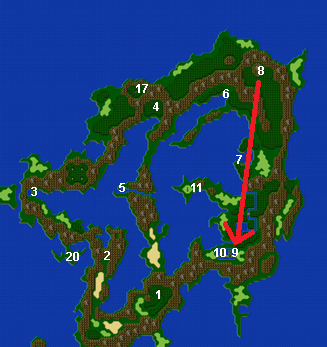
\includegraphics[scale=0.6]{../Graphics/Maps/1. To Walse.png}
\end{misc}

\switchcolumn*
\begin{enumerate}[resume]
    \item You can optionally loot the castle storage room for a \pickup{Tent, 490 Gil, and a Phoenix Down}
\end{enumerate}

\switchcolumn
\begin{misc}{Storage Room Optional Treasure}
    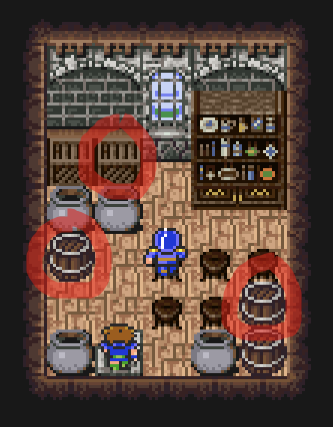
\includegraphics[scale=.399]{../Graphics/Misc/4. Walse Castle Optional Pickups.png}
\end{misc}

\switchcolumn
\resume
\begin{enumerate}[resume]
    \item Enter the throne room
    \item Head northwest to Walse Tower
    \item Grab the \pickup{Ether} in the bottom right corner on the last floor
\end{enumerate}

\begin{menu}{After Entering the Wind Crystal Shrine}
	\varwb
    \begin{jobMenu}
        \faris Knight \textbf{(A)}
        \galuf Blue Mage \textbf{(2\pointLeft)} \optimize
        \lenna Blue Mage \textbf{(2\pointLeft)} \optimize
        \bartz Blue Mage \textbf{(2\pointLeft)} \optimize
	\end{jobMenu}
    \begin{itemMenu}
        \potionMenu \ally{Faris (twice)}
    \end{itemMenu}
    \varwe
\end{menu}

\begin{boss}{Garula}
    \varwb
    \begin{round}{1 (Onwards)}
        \faris \leftCommand{\guard}
        \everyoneElse \leftCommand{\blue} \then \goblinPunch
    \end{round}
    \varwe
\end{boss}

\begin{menu}{Before Picking Up the Crystals}
	\varwb
    \begin{jobMenu}
        \bartz Thief \textbf{(2\pointRight)} \ability{!\black} \optimize
	\end{jobMenu}
    \varwe
\end{menu}

\end{paracol}
\chapter{Karnak}

\vspace{\baselineskip}

\begin{paracol}{2}

\begin{enumerate}
    \item Make your way to Karnak
\end{enumerate}

\switchcolumn
\begin{steproute}{En Route to Karnak}
    \insertStep{../Graphics/Steps/32. Karnak 1.jpg}
    \insertStep{../Graphics/Steps/33. Karnak 2.jpg}
    \insertStep{../Graphics/Steps/34. Karnak 3.jpg}
    \insertStep{../Graphics/Steps/35. Karnak 4.jpg}
\end{steproute}

\switchcolumn
\resume
\begin{enumerate}[resume]
    \item Head to the Armory
\end{enumerate}

\begin{shop}{Karnak Armory}
    \varwb
    \begin{sell}
        \item \shopHl{Everything Except}
        \begin{itemize}
            \item \tent
            \item \knife
            \item \phoenixDown
            \item \potion
        \end{itemize}
    \end{sell}
    \begin{buy}
        \item \shopHl{(5)} \iceRod \space \shopHl{x1}
    \end{buy}
    \varwe
\end{shop}

\switchcolumnTwice
\newpage
\begin{enumerate}[resume]
    \item Exit the castle
\end{enumerate}

\switchcolumn
\begin{steproute}{Karnak Castle}
    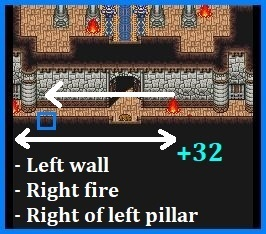
\includegraphics[scale=0.452]{../Graphics/Steps/36. Karnak 5.jpg}
\end{steproute}

\switchcolumn
\resume
\begin{enumerate}[resume]
    \item Return to the Armory
\end{enumerate}

\begin{shop}{Karnak Armory}
    \varwb
    \begin{buy}
        \item \shopHl{(5)} \iceRod \space \shopHl{x5}
    \end{buy}
    \varwe
\end{shop}

\begin{enumerate}[resume]
    \item Enter the steamship
\end{enumerate}

\end{paracol}
\chapter{Steamship}

\vspace{\baselineskip}

\begin{paracol}{2}

\vspace{-0.2cm}
\begin{enumerate}
    \item Grab the \pickup{Phoenix Down} by the world map
\end{enumerate}
\vspace{-0.2cm}

\switchcolumn
\begin{steproute}{Before the Menu}
    \insertStep{../Graphics/Steps/37. Steamship 1.jpg}
    \insertStep{../Graphics/Steps/38. Steamship 2.jpg}
\end{steproute}

\switchcolumn
\begin{menu}{After Activating the Far Right Level}
    \varwb
    \begin{itemMenu}
        \potionMenu \ally{Faris (twice)}
        \item \menuHl{Ensure Ice Rod is slot 1}
        \item[] 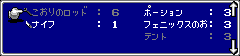
\includegraphics[scale=1.24]{../Graphics/Battle/3. Steamship Menu.png}
    \end{itemMenu}
    \begin{rowMenu}
        \swap Bartz \switch Galuf
    \end{rowMenu}
    \varwe
\end{menu}

\switchcolumn*
\begin{steproute}{Defeater x2 and CrewDust x2}
    \insertStep{../Graphics/Steps/39. Steamship Enc 1.jpg}
\end{steproute}

\switchcolumn
\begin{encounter}{Defeater x2 and CrewDust x2}
    \varwb
    \begin{notes}
        \item \encounterHl{Don't flee buffer}
        \item \encounterHl{You need to do inputs FAST}
    \end{notes}
    \begin{round}{1}
        \bartz Fight \then \ally{Galuf}
        \begin{notes}
            \item[] \encounterNote{(A)(\pointRight)(A)}
        \end{notes}
        \faris Defend
        \begin{notes}
            \item[] \encounterNote{(Hold R+A)}
        \end{notes}
        \lenna Item \then \battleGroup{Equip \iceRod} \then Break
        \begin{notes}
            \item[] \encounterNote{(\pointDown)(2A)(\pointUp)(3A)}
        \end{notes}
    \end{round}
    \varwe
\end{encounter}

\vspace{-0.25cm}
\begin{enumerate}[resume]
    \item Grab the \pickup{Elixir} before entering the boss room
\end{enumerate}
\vspace{-0.175cm}

\switchcolumn
\begin{steproute}{Before Liquid Flame}
    \insertStep{../Graphics/Steps/40. Steamship 3.jpg}
\end{steproute}

\switchcolumn
\begin{menu}{Before Liquid Flame}
    \varwb
    \begin{jobMenu}
        \lenna Time Mage \textbf{(\pointDown)} \optimize
        \faris Red Mage \textbf{(2\pointLeft)} \optimize
    \end{jobMenu}
    \begin{magicMenu}
        \faris \cure \space \then \ally{All to full}
    \end{magicMenu}
    \varwe
\end{menu}

\begin{boss}{Liquid Flame}
    \varwb
    \begin{round}{1}
        \bartz Item \then \battleGroup{Equip \knife} \then Defend
        \faris Item \then \battleGroup{\iceRod} \then Break
    \end{round}
    \begin{itemize}
        \item \newbox\hand \sbox\hand{\textbf{\ul{Round 2 (Hand)}}} \bossHl{{\usebox\hand}} 
        \begin{itemize}
            \lenna Defend
            \bartz Fight
            \faris
            \begin{itemize}
                \item \textit{If Lenna or Bartz died:} Item \then \battleGroup{\phoenixDown}
                \item \textit{Otherwise:} Item \then \battleGroup{Equip \iceRod } \then Break
            \end{itemize}
        \end{itemize}
    \end{itemize}
    \begin{itemize}
        \item \newbox\tornado \sbox\tornado{\textbf{\ul{Round 2 (Tornado)}}} \bossHl{{\usebox\tornado}} 
        \begin{itemize}
            \lenna Item \then \battleGroup{\iceRod} \then Break
        \end{itemize}
    \end{itemize}
    \varwe
\end{boss}

\end{paracol}
\chapter{Karnak Escape}

\vspace{\baselineskip}

\begin{paracol}{2}

\begin{enumerate}
    \item Use the pot to heal to full HP
    \item Grab the \pickup{2000 Gil} chest in the cell
\end{enumerate}

\switchcolumn
\begin{steproute}{After Getting the Chest}
    \insertStep{../Graphics/Steps/41. Karnak Escape 1 (Re-enter).jpg}
    \insertStep{../Graphics/Steps/42. Karnak Escape 2.jpg}
\end{steproute}

\switchcolumn*
\begin{enumerate}[resume]
    \item Grab these two \pickup{2000 Gil} chests in the upstairs rooms
\end{enumerate}

\switchcolumn
\begin{misc}{Upstairs Chests}
    \insertScreenshot{../Graphics/Misc/5. Karnak Chest 2.png}
    \insertScreenshot{../Graphics/Misc/6. Karnak Chest 3.png}
\end{misc}

\switchcolumnTwice*
\begin{steproute}{Before Sergeant}
    \insertStep{../Graphics/Steps/43. Karnak Escape 3.jpg}
\end{steproute}

\switchcolumn
\begin{boss}{Sergeant}
    \varwb
    \begin{round}{1}
        \bartz Defend
        \faris Item \then \battleGroup{Equip \iceRod} \then Break
        \item \bossHl{Don't queue the second Ice Rod until the Karnaks die}
        \lenna Item \then \battleGroup{\iceRod} \then Break
    \end{round}
    \varwe
\end{boss}

\begin{enumerate}[resume]
    \item Head back to Karnak
    \item Enter the magic shop
\end{enumerate}

\begin{shop}{Karnak Magic Shop}
    \varwb
    \begin{buy}[ (Left Wizard)]
        \item \shopHl{(2)} \life
    \end{buy}
    \varwe
\end{shop}

\begin{enumerate}[resume]
    \item Take the left door to the armory
\end{enumerate}

\begin{shop}{Karnak Armory Shop}
    \varwb
    \begin{itemize}
        \item \shopNote{Left Side}
    \end{itemize}
    \begin{buy}
        \item \shopHl{(6)} \silkRobe \space \shopHl{x1}
    \end{buy}
    \begin{itemize}
        \item \shopNote{Right Side}
    \end{itemize}
    \begin{buy}
        \item \shopHl{(1)} \mythrilKnife \space \shopHl{x1}
        \item \shopHl{(4)} \fireRod \space \shopHl{x2}
        \item \shopHl{(5)} \iceRod \space \shopHl{x1}
        \item \shopHl{(6)} \thunderRod \space \shopHl{x2}
    \end{buy}
    \varwe
\end{shop}    

\end{paracol}
\newpage

\chapter{Ancient Library}

\vspace{\baselineskip}

\begin{paracol}{2}

\begin{enumerate}
    \item Make your way to the Ancient Library
\end{enumerate}

\switchcolumn
\begin{steproute}{En Route to the Ancient Library}
    \insertStep{../Graphics/Steps/44. Karnak 10.jpg}
    \insertStep{../Graphics/Steps/45. En Route Ancient Library 1.jpg}
    \insertStep{../Graphics/Steps/46. En Route Ancient Library 2.jpg}
    \insertStep{../Graphics/Steps/47. En Route Ancient Library 3.jpg}
\end{steproute}

\switchcolumn
\resume
\begin{enumerate}[resume]
    \item If you need emergency healing you can use the left pot in the northern room
\end{enumerate}

\switchcolumnTwice[*]
\begin{boss}{Ifrit}
    \varwb
    \begin{round}{1}
        \bartz Wait
        \begin{itemize}
            \item \textit{If Ifrit kills Lenna/Faris:} Item \then \battleGroup{\phoenixDown}
            \item \textit{If Ifrit uses Flame:} \battleGroup{Defend}
        \end{itemize}
        \anyone
        \begin{itemize}
            \item \textit{If Bartz died:} Item \then \battleGroup{\phoenixDown}
            \item \textit{Otherwise:} Item \then \battleGroup{Equip \iceRod } \then Break
        \end{itemize}
        \anyone Item \then \battleGroup{Equip \iceRod } \then Break
    \end{round}
    \varwe
\end{boss}

\switchcolumn
\begin{steproute}{After Ifrit}
    \insertStep{../Graphics/Steps/48. Ancient Library 1.jpg}
\end{steproute}

\switchcolumn
\begin{enumerate}[resume]
    \item Grab the \pickup{Stealth Robe} in the downstairs library room
\end{enumerate}

\switchcolumn
\begin{steproute}{After Getting the Stealth Robe}
    \insertStep{../Graphics/Steps/49. Ancient Library 2.jpg}
\end{steproute}

\switchcolumn
\resume
\begin{enumerate}[resume]
    \item Grab the \pickup{Phoenix Down} in the dark room chest
\end{enumerate}

\switchcolumn*
\begin{steproute}{Before Byblos}
    \insertStep{../Graphics/Steps/50. Ancient Library 3.jpg}
    \insertStep{../Graphics/Steps/51. Ancient Library 4.jpg}
\end{steproute}

\switchcolumn
\begin{menu}{Before Byblos}
    \varwb
    \begin{itemMenu}
        \phoenixDownMenu \ally{Anyone dead}
    \end{itemMenu}
    \begin{magicMenu}
        \faris \cure \space \then \ally{All to full}
    \end{magicMenu}
    \begin{jobMenu}
        \faris Black Mage \textbf{(\pointDown)}
    \end{jobMenu}
    \varwe
\end{menu}

\begin{boss}{Byblos}
    \varwb
    \begin{round}{1}
        \bartz Wait
        \begin{itemize}
            \item \textit{If Byblos kills Galuf:} Item \then \battleGroup{\phoenixDown}
            \item \textit{Otherwise:} \battleGroup{Defend}
        \end{itemize}
        \lenna Item \then \battleGroup{Equip \fireRod } \then Break
        \faris Item \then \battleGroup{Equip \fireRod } \then Break
    \end{round}
    \begin{bossPart}{Menuing}
        \item \bossMenu{\textbf{Blank:} slot 1 \mbox{\pointRight} \textbf{Flame Scroll:} slot 3}
        \item \bossMenu{\textbf{Dagger:} down \mbox{\pointRight} \textbf{Ice Rods:} up}
        \vspace{1mm}
        \item[] \insertBattleMenu{../Graphics/Battle/4. Byblos Menu.png}
    \end{bossPart}
    \varwe
\end{boss}

\switchcolumnTwice[*]
\begin{menu}{After Byblos}
    \begin{jobMenu}
        \faris Ninja \textbf{(3\pointRight)} \equip{\stealthRobe}
        \lenna Mediator \textbf{(3\pointLeft)} \ability{!\black}
    \end{jobMenu}
\end{menu}

\switchcolumn
\begin{steproute}{After Byblos}
    \insertStep{../Graphics/Steps/52. Ancient Library 5.jpg}
    \insertStep{../Graphics/Steps/53. Ancient Library Enc 1.jpg}
\end{steproute}

\switchcolumn
\begin{encounter}{Page 64}
	\varwb
	\begin{notes}
		\item \encounterHl{Don't flee buffer}
	\end{notes}
	\begin{round}{1}
		\faris \leftCommand{\throw} \then \broadsword
        \bartz Defend
        \lenna \rightCommand{\black} \then \fire
        \galuf Defend
	\end{round}
    \begin{round}{2 (Onwards)}
		\faris \leftCommand{\throw} \then \mythrilKnife
        \bartz Defend
        \item Wait until he uses L.5 Death
        \lenna \leftCommand{\catch}
	\end{round}
	\varwe
\end{encounter}

\end{paracol}
\chapter{Karnak Revisit}

\vspace{\baselineskip}

\begin{paracol}{2}

\begin{enumerate}
    \item Head back to Karnak
\end{enumerate}

\switchcolumn
\begin{steproute}{En Route to Karnak}
    \insertStep{../Graphics/Steps/54. Karnak 1.jpg}
    \insertStep{../Graphics/Steps/55. Karnak 2.jpg}
    \insertStep{../Graphics/Steps/56. Karnak 3.jpg}
    \insertStep{../Graphics/Steps/57. Karnak 4.jpg}
\end{steproute}

\switchcolumn
\resume
\begin{enumerate}[resume]
    \item Make your way to the pub
\end{enumerate}

\switchcolumnTwice
\begin{enumerate}[resume]
    \item Enter the steamship after the cutscenes
\end{enumerate}

\switchcolumn
\begin{steproute}{Before Steamship}
    \insertStep{../Graphics/Steps/58. Karnak 5.jpg}
\end{steproute}

\end{paracol}
\chapter{Crescent}

\vspace{\baselineskip}

\begin{paracol}{2}

\begin{enumerate}
    \item Start travelling towards Crescent
\end{enumerate}

\switchcolumn
\begin{misc}{Path to Crescent}
    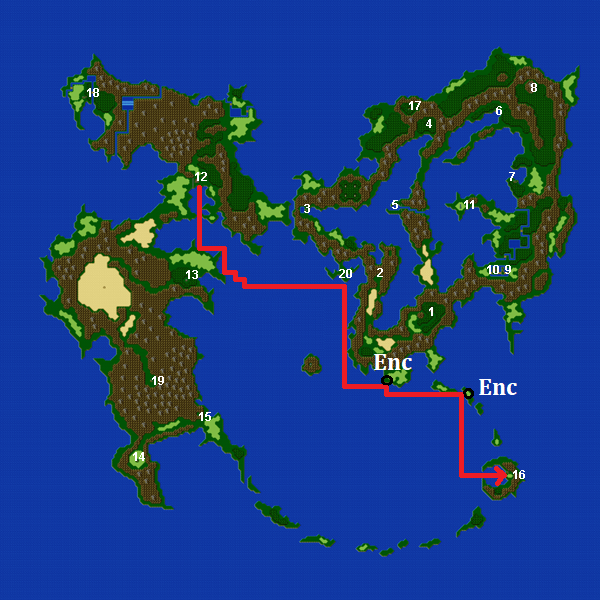
\includegraphics[scale=0.8]{../Graphics/Maps/2. To Crescent.png}
\end{misc}

\switchcolumn*
\begin{enumerate}[resume]
    \item Disembark at the following landmass and fight two encounters
\end{enumerate}

\switchcolumn
\begin{steproute}{Black Flame Island}
    \insertStep{../Graphics/Steps/59. Crescent Enc 1.jpg}
\end{steproute}

\switchcolumn
\begin{encounter}{Black Flame x5}
	\varwb
	\begin{notes}
		\item \encounterHl{Don't flee buffer}
		\item \encounterHl{Flame Scroll (\pointUp)}
	\end{notes}
	\begin{round}{1}
		\faris \leftCommand{\throw} \then \flameScroll
	\end{round}
	\varwe
\end{encounter}

\begin{menu}{After the First Black Flame Encounter}
    \varwb
    \begin{jobMenu}
        \lenna Time Mage \textbf{(\pointDown)(\pointRight)} \optimize
    \end{jobMenu}
    \begin{itemMenu}
        \potionMenu \ally{If necessary}
    \end{itemMenu}
    \varwe
\end{menu}

\begin{encounter}{Black Flame x5}
	\varwb
	\begin{notes}
		\item \encounterHl{Don't flee buffer}
		\item \encounterHl{Thunder Rod is already equipped}
	\end{notes}
	\begin{round}{1}
		\faris Defend
        \bartz Defend
        \lenna Item \then \battleGroup{\thunderRod} \then Break
	\end{round}
	\varwe
\end{encounter}

\begin{enumerate}[resume]
    \item Enter Crescent
\end{enumerate}

\end{paracol}
\chapter{Lix}

\vspace{\baselineskip}

\begin{paracol}{2}

\begin{enumerate}
    \item After the cutscene, head to the forest
    \item After catching the chocobo, head to Lix
\end{enumerate}

\switchcolumn
\begin{misc}{Path to Lix}
    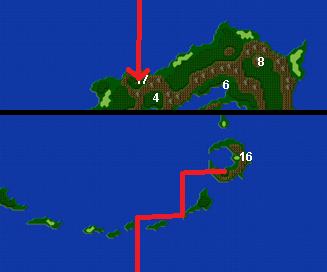
\includegraphics[scale=1.45]{../Graphics/Maps/3. To Lix.png}
\end{misc}

\switchcolumn
\resume
\begin{enumerate}[resume]
    \item Head to the multipurpose sales building (2nd floor)
\end{enumerate}

\begin{menu}{Before the Shop}
    \varwb
    \begin{jobMenu}
        \lenna Ninja \textbf{(3\pointRight)} \ability{!\black}
        \galuf Ninja \textbf{(3\pointRight)} \ability{!\observe}
        \faris Ninja \textbf{(3\pointRight)} \ability{!\black}
    \end{jobMenu}
    \varwe
\end{menu}

\begin{shop}{Lix Shop}
    \varwb
    \begin{sell}
        \item \shopHl{Everything Except}
        \begin{itemize}
            \item \potion
            \item \silkRobe
            \item \elixir
            \item \thunderRod
        \end{itemize}
    \end{sell}
    \begin{buy}
        \item \shopHl{(1)} \kunai \space \shopHl{x1}
        \item \shopHl{(4)} \waterScroll \space \shopHl{x5}
        \item \shopHl{(5)} \thunderScroll \space \shopHl{x27}
    \end{buy}
    \varwe
\end{shop}

\begin{enumerate}[resume]
    \item Exit from the top and make your way to the Ancient Library
\end{enumerate}

\switchcolumn
\begin{misc}{Path to the Ancient Library}
    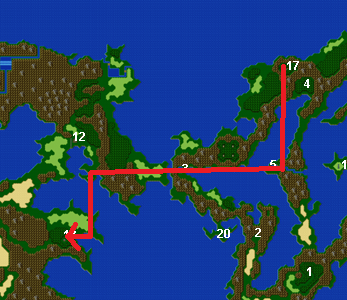
\includegraphics[scale=0.6]{../Graphics/Maps/4. To Ancient Library.png}
\end{misc}

\switchcolumn
\begin{enumerate}[resume]
    \item After the cutscenes, head to the desert
\end{enumerate}

\end{paracol}
\newpage
\chapter{Quicksand Desert}

\vspace{\baselineskip}

\begin{paracol}{2}

\begin{boss}{Sandworm}
    \varwb
    \begin{round}{1}
        \bartz Defend
        \faris Item \then \battleGroup{Equip \kunai} \then \leftCommand{\throw} \then \waterScroll
        \lenna \leftCommand{\throw} \then \waterScroll
        \item \bossMenu{\textbf{Thunder Scrolls:} slot 1}
        \vspace{1mm}
        \item[] \insertBattleMenu{../Graphics/Battle/5. Sandworm Menu.png}
        \galuf \leftCommand{\throw} \then \waterScroll
    \end{round}
    \varwe
\end{boss}

\switchcolumnTwice[*]
\begin{menu}{After Sandworm}
    \varwb
    \begin{jobMenu}
        \galuf White Mage \textbf{(\pointDown)}
        \lenna Mediator \textbf{(\pointDown)(\pointLeft)(\pointDown)}
    \end{jobMenu}
    \begin{magicMenu}
        \galuf \cure \space \then \ally{All to full}
    \end{magicMenu}
    \varwe
\end{menu}

\begin{encounter}{Sand Killer x2 (x2)}
	\varwb
	\begin{notes}
		\item \encounterHl{Hold A entering the encounters}
	\end{notes}
	\begin{round}{1}
		\faris \leftCommand{\throw} \then \waterScroll
	\end{round}
	\varwe
\end{encounter}

\switchcolumn
\newpage
\begin{steproute}{Quicksand Desert Encounters}
    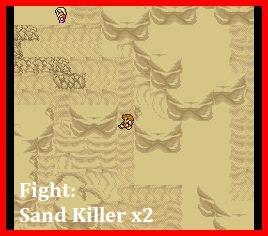
\includegraphics[scale=0.448]{../Graphics/Steps/66. Quicksand Enc 1.jpg}
    \insertStep{../Graphics/Steps/67. Quicksand Enc 2.jpg}
\end{steproute}

\switchcolumn*
\begin{enumerate}
    \item Follow this path through the desert
\end{enumerate}

\switchcolumn
\begin{misc}{Desert Path}
    \insertMisc{../Graphics/Misc/7. Quicksand 1.png}
    \insertMisc{../Graphics/Misc/8. Quicksand 2.png}
    \insertMisc{../Graphics/Misc/9. Quicksand 3.png}
\end{misc}

\switchcolumn*
\resume
\begin{enumerate}[resume]
    \item Head towards the Ancient Ruins
\end{enumerate}

\switchcolumn
\begin{steproute}{Before Ancient Ruins}
    \insertStep{../Graphics/Steps/68. Ancient Ruins 1.jpg}
    \insertStep{../Graphics/Steps/69. Ancient Ruins 2.jpg}
\end{steproute}

\switchcolumn
\resume
\begin{enumerate}[resume]
    \item Move to the front of the stairs
    \item Lure Tycoon northwest
    \item Corner him in the building in the centre
    \item On the airship, follow Cid downstairs when they leave
    \item Talk to Cid a second time once you regain control
\end{enumerate}

\begin{boss}{Crayclaw}
    \varwb
    \begin{round}{1}
        \faris \leftCommand{\throw} \then \thunderScroll
        \bartz Defend
        \lenna \leftCommand{\release}
    \end{round}
    \varwe
\end{boss}

\end{paracol}
\chapter{Airship Sequence}

\vspace{\baselineskip}

\begin{paracol}{2}

\begin{enumerate}
    \item Fly to the Ancient Ruins
    \item Fly back to Crescent HQ and talk to Cid
\end{enumerate}

\switchcolumn
\begin{misc}{Path to the Ancient Ruins}
    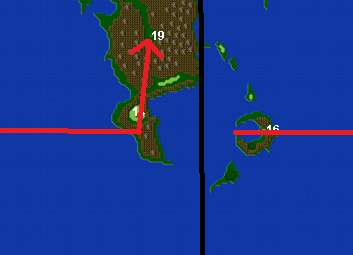
\includegraphics[scale=0.7]{../Graphics/Maps/5. To Ruins.png}
\end{misc}

\switchcolumn*
\resume
\begin{enumerate}[resume]
    \item Fly to the Tycoon Meteor, stopping at the following island along the way
\end{enumerate}

\switchcolumn
\begin{misc}{Path to the Tycoon Meteor}
    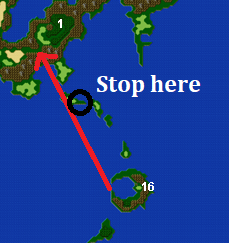
\includegraphics[scale=1.45]{../Graphics/Maps/6. To Tycoon Meteor.png}
\end{misc}

\switchcolumn
\begin{encounter}{Black Flame x5}
	\varwb
	\begin{notes}
		\item \encounterHl{Hold A entering the encounter}
	\end{notes}
	\begin{round}{1}
		\faris \leftCommand{\throw} \then \thunderScroll
	\end{round}
	\varwe
\end{encounter}

\begin{menu}{After the First Black Flame Encounter}
    \varwb
    \begin{jobMenu}
        \galuf Thief \textbf{(2\pointRight)} \ability{!\white}
        \bartz Bard \textbf{(\pointUp)}
    \end{jobMenu}
    \varwe
\end{menu}

\begin{encounter}{Black Flame x5 (x2)}
	\varwb
	\begin{notes}
		\item \encounterHl{Hold A entering the encounters}
	\end{notes}
	\begin{round}{1}
		\faris \leftCommand{\throw} \then \thunderScroll
	\end{round}
	\varwe
\end{encounter}

\begin{enumerate}[resume]
    \item At the Tycoon Meteor, grab the hidden \pickup{Phoenix Down} on the right
\end{enumerate}

\begin{menu}{Before Adamantoise}
    \varwb
    \begin{jobMenu}
        \bartz Blue Mage \textbf{(\pointDown)(4\pointRight)} \optimize
    \end{jobMenu}
    \begin{magicMenu}
        \galuf \cure \space \then \ally{Bartz to full}
    \end{magicMenu}
    \varwe
\end{menu}

\begin{boss}{Adamantoise}
	\varwb
	\begin{round}{1}
		\faris Defend
        \galuf Defend
        \lenna Defend
        \bartz \leftCommand{\blue} \then \lfiveDeath
	\end{round}
	\varwe
\end{boss}

\begin{enumerate}[resume]
    \item Fly back to Crescent HQ and talk to Cid
    \item Ascend up into the air
    \item Reminder that you can dash with the airship
\end{enumerate}

\begin{menu}{Before the First Rocket Fight}
    \varwb
    \begin{jobMenu}
        \bartz Bard \textbf{(\pointUp)} \ability{!\black}
        \lenna Ninja \textbf{(3\pointRight)} \ability{!\black}
    \end{jobMenu}
    \varwe
\end{menu}

\begin{encounter}{Rockets x2 or Flamegun x2 (x4)}
	\varwb
	\begin{notes}
		\item \encounterHl{You can flee buffer these encounters}
	\end{notes}
	\begin{round}{1}
		\faris \leftCommand{\throw} \then \thunderScroll
        \galuf Defend
        \lenna \leftCommand{\throw} \then \thunderScroll
        \bartz \rightCommand{\black} \then \bolt \space \then \enemy{All}
	\end{round}
	\varwe
\end{encounter}

\begin{menu}{Before Soul Cannon}
    \varwb
    \begin{jobMenu}
        \galuf Ninja \textbf{(3\pointRight)} \ability{!\white}
    \end{jobMenu}
    \varwe
\end{menu}

\begin{boss}{Soul Cannon}
	\varwb
	\begin{round}{1}
        \faris \leftCommand{\throw} \then \thunderScroll
        \lenna \leftCommand{\throw} \then \thunderScroll
        \galuf \leftCommand{\throw} \then \thunderScroll
        \bartz \rightCommand{\black} \then \bolt
	\end{round}
    \begin{round}{2 (Onwards)}
        \bartz \rightCommand{\black} \then \bolt
        \everyoneElse \leftCommand{\throw} \then \thunderScroll
	\end{round}
	\varwe
\end{boss}

\begin{menu}{After Soul Cannon}
    \varwb
    \begin{jobMenu}
        \faris Geomancer \textbf{(\pointUp)(\pointLeft)}
        \bartz Thief \textbf{(2\pointRight)} \ability{!\escape}
    \end{jobMenu}
    \varwe
\end{menu}

\end{paracol}
\chapter{Lonka Ruins}

\vspace{\baselineskip}

\begin{paracol}{2}

\begin{enumerate}
    \item \battleGroup{Escape is the right command}
    \item Grab the \pickup{Gold Armor} chest on the 2nd screen
\end{enumerate}

\switchcolumn
\begin{misc}{Before HiPotion Chest}
    \insertStep {../Graphics/Steps/76. Lonka Ruins 2.jpg}
\end{misc}

\switchcolumn
\resume
\begin{enumerate}[resume]
    \item Grab the \pickup{HiPotion} after this screen
\end{enumerate}

\switchcolumn
\begin{misc}{Before Treasure Room}
    \insertStep{../Graphics/Steps/77. Lonka Ruins 3.jpg}
\end{misc}

\switchcolumn
\newpage
\begin{enumerate}[resume]
    \item Grab all five chests in the treasure room: \pickup{Shuriken, 5000 Gil, Ancient Sword, Full Moon, and Power Ring}
\end{enumerate}

\switchcolumn
\begin{misc}{Treasure Room}
    \insertMisc{../Graphics/Misc/10. Lonka Ruins Chests.png}
\end{misc}

\switchcolumn*
\begin{enumerate}[resume]
    \item Grab the \pickup{Cabin} and \pickup{Ether} chests after this screen
\end{enumerate}

\switchcolumn
\begin{misc}{Before Cabin and Ether Chests}
    \insertStep{../Graphics/Steps/82. Lonka Ruins 7.jpg}
\end{misc}

\switchcolumn
\begin{menu}{Before Archeoaevis}
    \varwb
    \begin{notes}
        \item \menuHl{Heal if necessary}
    \end{notes}
    \begin{jobMenu}
        \bartz Blue Mage \textbf{(\pointDown)(4\pointRight)} \optimize \space \equip{\thunderRod}
    \end{jobMenu}
    \varwe
\end{menu}

\begin{boss}{Archeoaevis}
	\varwb
	\begin{round}{1}
		\lenna \leftCommand{\throw} \then \thunderScroll
        \galuf Defend
        \item \bossHl{Don't run buffer Faris or Bartz's turns}
        \item \bossHl{Lenna should be nearly at full ATB after Bartz's turn}
        \faris \leftCommand{\gaia}
        \bartz Item \then \battleGroup{\thunderRod} \then Break
	\end{round}
    \begin{round}{2}
        \lenna \leftCommand{\throw} \then \thunderScroll
        \galuf Defend
        \faris \leftCommand{\gaia}
        \lenna \leftCommand{\throw} \then \thunderScroll
        \bartz Defend
    \end{round}
    \begin{round}{3}
        \galuf \leftCommand{\throw} \then \thunderScroll
        \faris \leftCommand{\gaia}
        \lenna \leftCommand{\throw} \then \shuriken
        \galuf \leftCommand{\throw} \then \ancientSword
    \end{round}
    \begin{round}{4 (After Transition)}
        \bartz \leftCommand{\blue} \then \lfiveDeath
    \end{round}
	\varwe
\end{boss}

\begin{menu}{After Archeoaevis}
    \varwb
    \begin{jobMenu}
        \lenna Thief \textbf{(2\pointRight)} \ability{!\tame}
        \galuf Thief \textbf{(2\pointRight)}
    \end{jobMenu}
    \varwe
\end{menu}

\end{paracol}
\newpage
\chapter{Meteor Fetch}

\vspace{\baselineskip}

\begin{paracol}{2}

\begin{enumerate}
    \item Head to the Tycoon Meteor
\end{enumerate}

\switchcolumn
\begin{misc}{Path to the Tycoon Meteor}
    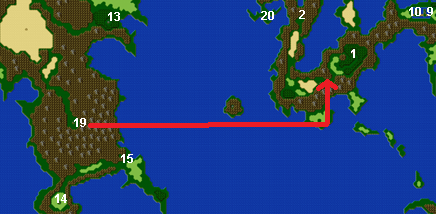
\includegraphics[scale=0.75]{../Graphics/Maps/7. To Tycoon Meteor.png}
\end{misc}

\switchcolumn*
\begin{enumerate}[resume]
    \item Head to the Walse Meteor
\end{enumerate}

\switchcolumn
\begin{misc}{Path to the Walse Meteor}
    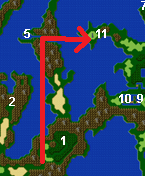
\includegraphics{../Graphics/Maps/8. To Walse Meteor.png}
\end{misc}

\switchcolumn*
\begin{menu}{Before Talking to Cid}
    \varwb
    \begin{jobMenu}
        \faris Samurai \textbf{(\pointLeft)(\pointDown)}
        \bartz Samurai \textbf{(\pointLeft)(\pointDown)} \ability{!\hide}
    \end{jobMenu}
    \varwe
\end{menu}

\switchcolumnTwice[*]
\begin{boss}{Puroboros}
	\varwb
	\begin{round}{1}
		\lenna Defend
        \faris \leftCommand{\gilToss}
        \item \bossMenu{\textbf{Potions:} down \mbox{\pointRight} \textbf{Ethers:} up \mbox{\pointRight} \textbf{Ice Bow:} up}
        \item \bossMenu{\textbf{Hero Drink:} slot 3 \mbox{\pointRight} \textbf{Phoenix Downs:} slot 4}
        \vspace{1mm}
        \item[] \insertBattleMenu{../Graphics/Battle/6. Puroboros Menu.png}
    \end{round}
	\varwe
\end{boss}

\begin{enumerate}[resume]
    \item Head to the Ruins Meteor
\end{enumerate}

\switchcolumn
\begin{misc}{Path to the Ruins Meteor}
    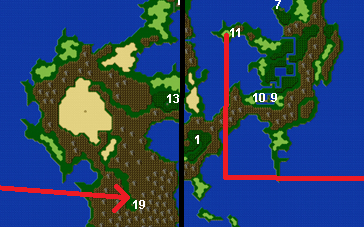
\includegraphics[scale=1.15]{../Graphics/Maps/9. To Ruins Meteor.png}
\end{misc}

\switchcolumn*
\begin{boss}{Chimera Brain}
	\varwb
	\begin{round}{1}
		\lenna \rightCommand{\tame}
        \faris \leftCommand{\gilToss}
        \bartz \leftCommand{\gilToss}
    \end{round}
	\varwe
\end{boss}

\begin{enumerate}[resume]
    \item Head to the Karnak Meteor
\end{enumerate}

\switchcolumn
\begin{misc}{Path to the Karnak Meteor}
    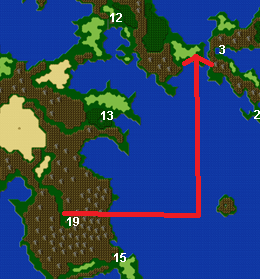
\includegraphics[scale=0.532]{../Graphics/Maps/10. To Karnak Meteor.png}
\end{misc}

\begin{misc}{Menu Here}
    \insertScreenshot{../Graphics/Misc/11. Titan Menu.png}
\end{misc}

\switchcolumn
\begin{menu}{Before Titan}
    \varwb
    \begin{jobMenu}
        \lenna Ninja \textbf{(2\pointLeft)(\pointDown)} \ability{!\black}
    \end{jobMenu}
    \varwe
\end{menu}

\begin{boss}{Titan}
	\varwb
	\begin{round}{1}
		\lenna Defend
        \faris \leftCommand{\gilToss}
        \bartz \rightCommand{\hide}
        \lenna \leftCommand{\throw} \then \thunderScroll
    \end{round}
	\varwe
\end{boss}

\begin{menu}{After Titan}
    \varwb
    \begin{jobMenu}
        \bartz Thief \textbf{(2\pointRight)} \optimize
    \end{jobMenu}
    \begin{itemMenu}
        \item \menuHl{Previous menuing if required}
        \item[] \insertBattleMenu{../Graphics/Battle/6. Puroboros Menu.png}
    \end{itemMenu}
    \varwe
\end{menu}

\begin{enumerate}[resume]
    \item Head southeast to the portal
\end{enumerate}

\end{paracol}
\chapter{World Two}

\vspace{\baselineskip}

\begin{paracol}{2}

\begin{menu}{After Gaining Control}
    \varwb
    \begin{itemMenu}
        \item \cottage
    \end{itemMenu}
    \varwe
\end{menu}

\begin{boss}{Abductor}
	\varwb
	\begin{round}{1}
		\bartz Fight \then \ally{Bartz}
    \end{round}
	\varwe
\end{boss}

\switchcolumn*
\begin{misc}{Menu Here}
    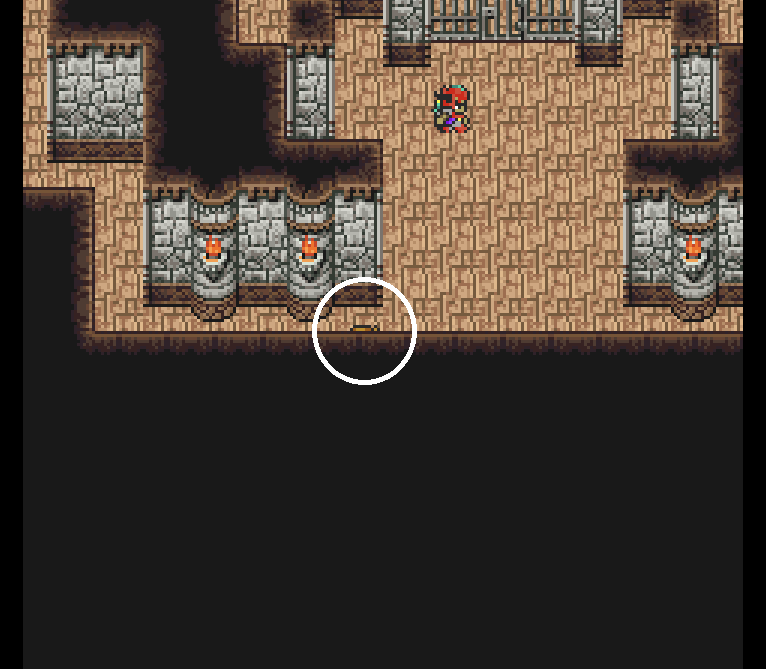
\includegraphics[scale=0.157]{../Graphics/Misc/12. Gilgamesh Menu.png}
\end{misc}

\switchcolumn
\begin{menu}{Before Reaching Gilgamesh}
    \varwb
    \begin{jobMenu}
        \galuf Samurai \textbf{(\pointLeft)(\pointDown)} \ability{!\white}
    \end{jobMenu}
    \varwe
\end{menu}

\begin{boss}{Gilgamesh}
	\varwb
	\begin{round}{1}
        \galuf \leftCommand{\gilToss}
    \end{round}
	\varwe
\end{boss}

\begin{enumerate}
    \item Make your way to the Big Bridge
\end{enumerate}

\begin{encounter}{Lil' Chariot x3}
	\varwb
	\begin{round}{1}
		\bartz Defend
        \lenna \leftCommand{\throw} \then \thunderScroll
    \end{round}
	\varwe
\end{encounter}

\begin{enumerate}[resume]
    \item Left until the 2nd tower then right until the chamber
\end{enumerate}

\switchcolumn*
\begin{misc}{Menu Here}
    \insertScreenshot{../Graphics/Misc/13. Gilagmesh 2 Menu.png}
\end{misc}

\switchcolumn
\begin{menu}{Before Gilgamesh}
    \varwb
    \begin{jobMenu}
        \lenna Samurai \textbf{(\pointLeft)(\pointDown)} \optimize
        \bartz Samurai \textbf{(\pointLeft)(\pointDown)}
    \end{jobMenu}
    \begin{magicMenu}
        \galuf \cure \space \then \ally{All to full}
    \end{magicMenu}
    \varwe
\end{menu}

\begin{boss}{Gilgamesh}
	\varwb
	\begin{round}{1}
        \faris Defend
        \lenna \leftCommand{\gilToss}
        \bartz \leftCommand{\gilToss}
        \galuf \leftCommand{\gilToss}
    \end{round}
    \begin{round}{2 (Onwards)}
        \faris Wait for Lenna's ATB \then \leftCommand{\gilToss}
        \item \bossMenu{\textbf{Phoenix Downs:} slot 6 \mbox{\pointRight} \textbf{HiPotions:} slot 2}
        \item \bossMenu{Move other items down 2-3 rows to make space}
        \vspace{1mm}
        \item[] \insertBattleMenu{../Graphics/Battle/7. Gilgamesh Menu.png}
        \lenna \leftCommand{\gilToss} 
        \anyone \leftCommand{\gilToss}
        \anyone \leftCommand{\gilToss}
    \end{round}
	\varwe
\end{boss}

\switchcolumnTwice[*]
\begin{menu}{After Gilgamesh}
    \varwb
    \begin{jobMenu}
        \bartz White Mage \textbf{(\pointDown)(2\pointRight)}
    \end{jobMenu}
    \begin{magicMenu}
        \bartz \life \space \then \ally{Anyone dead}
        \bartz \cure \space \then \ally{All to full}
    \end{magicMenu}
    \begin{jobMenu}
        \bartz Thief \textbf{(2\pointRight)} \ability{!\escape}
    \end{jobMenu}
    \varwe
\end{menu}

\begin{enumerate}[resume]
    \item Left until just before the 2nd tower and then do this movement
\end{enumerate}

\switchcolumn
\begin{misc}{Big Bridge Movement}
    \insertScreenshot{../Graphics/Misc/14. Big Bridge Movement.png}
\end{misc}

\end{paracol}
\chapter{Grociana}

\vspace{\baselineskip}

\begin{paracol}{2}

\begin{enumerate}
    \item Make your way towards the underground
\end{enumerate}

\switchcolumn
\begin{steproute}{En Route to the Underground}
    \insertStep{../Graphics/Steps/91. Grociana 1.jpg}
    \insertStep{../Graphics/Steps/92. Grociana 2.jpg}
    \insertStep{../Graphics/Steps/93. Grociana 3.jpg}
    \insertStep{../Graphics/Steps/94. Grociana Enc 1.jpg}
    \insertStep{../Graphics/Steps/95. Grociana 4.jpg}
    \insertStep{../Graphics/Steps/96. Grociana 5.jpg}
    \insertStep{../Graphics/Steps/97. Grociana 6.jpg}
    \insertStep{../Graphics/Steps/98. Grociana 7.jpg}
    \insertStep{../Graphics/Steps/99. Grociana 8.jpg}
    \insertStep{../Graphics/Steps/100. Grociana 9.jpg}
    \insertStep{../Graphics/Steps/101. Grociana 10.jpg}
\end{steproute}

\switchcolumnTwice[*]
\begin{steproute}{After the Chest}
    \insertStep{../Graphics/Steps/102. Underground 1.jpg}
\end{steproute}

\switchcolumn
\begin{enumerate}[resume]
    \item Grab the \pickup{4400 Gil} chest along the way
\end{enumerate}

\begin{menu}{Before Tyrasaurus}
    \varwb
    \begin{jobMenu}
        \bartz Samurai \textbf{(\pointLeft)(\pointDown)}
        \lenna Mediator \textbf{(\pointUp)}
        \galuf Thief \textbf{(2\pointRight)}
    \end{jobMenu}
    \begin{itemMenu}
        \hiPotionMenu \ally{People missing 100+ HP (two max)}
    \end{itemMenu}
    \varwe
\end{menu}

\begin{boss}{Tyrasaurus}
    \varwb
    \begin{round}{1 (Onwards)}
        \everyone \phoenixDown \space \then \enemy{Tyrasaurus}
    \end{round}
    \begin{itemize}
        \item \newbox\backup \sbox\backup{\textbf{\ul{If You Run Out of Phoenix Downs}}} \bossHl{{\usebox\backup}} 
        \begin{itemize}
            \anyone \elixir \space \then \enemy{Tyrasaurus}
            \anyone \potion \space \then \enemy{Tyrasaurus}
        \end{itemize}
    \end{itemize}
    \varwe
\end{boss}

\newpage
\begin{enumerate}[resume]
    \item Head toward Moogle Village
\end{enumerate}

\switchcolumn
\begin{steproute}{En Route to Moogle Village}
    \insertStep{../Graphics/Steps/103. Moogle Village 1.jpg}
    \insertStep{../Graphics/Steps/104. Moogle Village 2.jpg}
    \insertStep{../Graphics/Steps/105. Moogle Village 3.jpg}
    \insertStep{../Graphics/Steps/106. Moogle Village 4.jpg}
    \insertStep{../Graphics/Steps/107. Moogle Village 5.jpg}
    \insertStep{../Graphics/Steps/108. Moogle Village 6.jpg}
    \insertStep{../Graphics/Steps/109. Moogle Village 7.jpg}
    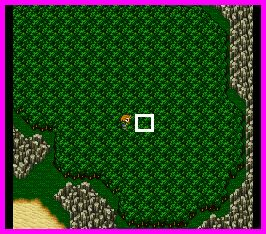
\includegraphics[scale=0.449]{../Graphics/Steps/110. Moogle Village 8.jpeg}
\end{steproute}

\switchcolumn*
\begin{enumerate}[resume]
    \item Head to the top right of the village and talk to the moogle to start the internal timer
    \item Talk to the moogle inside the tree
    \item Grab all the chests except the top right one: \pickup{Cabin, Dancing Dagger, 10000 Gil, Phoenix Down, and Ether}
\end{enumerate}

\switchcolumn
\begin{misc}{Moogle Village Chests}
    \insertMisc{../Graphics/Misc/15. Moogle Village Chests.png}
\end{misc}

\end{paracol}
\chapter{Dragon Valley}

\vspace{\baselineskip}

\begin{paracol}{2}

\begin{enumerate}
    \item Grab the \pickup{Exit} spell in the bottom left of the throne room
    \item Go to Cara on the rooftop
    \item Make your way to Kelb
\end{enumerate}

\begin{boss}{Abductor}
	\varwb
	\begin{round}{1}
		\galuf Defend
        \faris \leftCommand{\gilToss}
    \end{round}
	\varwe
\end{boss}

\begin{menu}{After Abductor}
    \varwb
    \begin{itemMenu}
        \hiPotionMenu \ally{Whoever was hit by Abductor}
    \end{itemMenu}
    \begin{jobMenu}
        \bartz Thief \textbf{(2\pointRight)} \ability{!\escape} \optimize
    \end{jobMenu}
    \varwe
\end{menu}

\begin{enumerate}[resume]
    \item Enter the biggest mansion, walk one tile inside, then leave
    \item Head north to Dragon Valley
\end{enumerate}

\switchcolumn*
\begin{steproute}{Extra Chest}
    Grab the \pickup{5000 Gil} chest in the cave on the first screen
\end{steproute}

\switchcolumn
\resume
\begin{enumerate}[resume]
    \item Grab the \pickup{Bone Mail} on the pile of bones
    \item Grab the \pickup{7000 Gil} after activating the switch
    \item Grab the \pickup{Coronet} and \pickup{Air Blade} southern part of the cave
    \item Grab the \pickup{Phoenix Down} before exiting the last cave
\end{enumerate}

\begin{menu}{Before Hiryuu Plant}
    \varwb
    \begin{jobMenu}
        \bartz Samurai \textbf{(\pointLeft)(\pointDown)} \equip{\dancingDagger}
    \end{jobMenu}
    \varwe
\end{menu}

\begin{boss}{Hiryuu Plant}
    \varwb
    \begin{round}{1}
        \galuf Defend
        \faris \leftCommand{\gilToss}
        \bartz \leftCommand{\gilToss}
        \item \bossMenu{\textbf{Gold Armor:} slot 1 \mbox{\pointRight} \textbf{Power Wrist:} up}
        \vspace{1mm}
        \item[] \insertBattleMenu{../Graphics/Battle/8. Hiryuu Menu.png}
        \lenna Defend
    \end{round}
    \begin{round}{2}
        \galuf Defend
        \faris \leftCommand{\gilToss}
        \bartz \leftCommand{\gilToss}
    \end{round}
    \varwe
\end{boss}

\begin{menu}{After Hiryuu Plant}
    \varwb
    \begin{jobMenu}
        \faris Time Mage \textbf{(2\pointLeft)(\pointUp)}
    \end{jobMenu}
    \begin{magicMenu}
        \faris \exit
    \end{magicMenu}
    \varwe
\end{menu}

\end{paracol}
\chapter{Kelb}

\vspace{\baselineskip}

\begin{paracol}{2}

\begin{enumerate}
    \item Make your way back to Kelb
    \item Go to the Magic Shop
\end{enumerate}

\begin{shop}{Kelb Magic Shop}
    \varwb
    \begin{buy}
        \item \textit{Right Wolf}
        \begin{itemize}
            \item \shopHl{(3)} \reset
        \end{itemize}
        \item \textit{Left Wolf}
        \item \begin{itemize}
            \item \shopHl{(2)} \breakSpell
        \end{itemize}
    \end{buy}
    \varwe
\end{shop}

\begin{enumerate}[resume]
    \item Go to the Armory
\end{enumerate}

\begin{shop}{Kelb Armory}
    \varwb
    \begin{sell}
        \item \goldArmor
        \item \iceBow
        \item \powerWrist
        \item \silkRobe
        \item \ether
    \end{sell}
    \begin{buy}
        \item \textit{Right Side, Left Wolf}
        \begin{itemize}
            \item \shopHl{(5)} \flameScroll \space \shopHl{(x4)}
            \item \shopHl{(7)} \thunderScroll \space \shopHl{(x11)}
        \end{itemize}
        \item \textit{Left Side, Right Wolf}
        \begin{itemize}
            \item \shopHl{(3)} \greenBeret \space \shopHl{(x1)}
            \item \shopHl{(6)} \stealthRobe \space \shopHl{(x1)}
        \end{itemize}
    \end{buy}
    \varwe
\end{shop}

\begin{enumerate}[resume]
    \item Go to the Inn
\end{enumerate}

\begin{menu}{Before the Inn Shop}
    \varwb
    \begin{jobMenu}
        \faris Ninja \textbf{(\pointLeft)(\pointDown)(\pointLeft)} \optimize
    \end{jobMenu}
    \varwe
\end{menu}

\begin{shop}{Kelb Inn}
    \varwb
    \begin{buy}
        \item \textit{Bottom Wolf}
        \begin{itemize}
            \item \shopHl{(6)} \speedDrink \space \shopHl{(x1)}
            \item \shopHl{(8)} \heroDrink \space \shopHl{(x3)}
            \item \shopHl{(2)} \revivify \space \shopHl{(x1)}
        \end{itemize}
        \item \textit{Top Wolf}
        \item \begin{itemize}
            \item \shopHl{(1)} \hiPotion \space \shopHl{(x11)}
            \item \shopHl{(8)} \antidote \space \shopHl{(x11)}
            \item \shopHl{(7)} \eyedrop \space \shopHl{(x11)}
            \item \shopHl{(5)} \maidensKiss \space \shopHl{(x2)}
        \end{itemize}
    \end{buy}
    \begin{itemize}
        \item \shopNote{You need to have less than 1500 Gil leaving the shop}
    \end{itemize}
    \varwe
\end{shop}

\begin{enumerate}[resume]
    \item Start heading towards Bal
\end{enumerate}

\begin{menu}{Before the Encounter}
    \varwb
    \begin{itemMenu}
        \antidoteMenu \ally{Anyone poisoned}
        \hiPotionMenu \ally{Anyone low on HP}
    \end{itemMenu}
    \varwe
\end{menu}

\begin{enumerate}[resume]
    \item Search for the Kornago, Weresnake, Aquathone encounter
\end{enumerate}

\begin{encounter}{Kornago, Weresnake, Aquathone (150 EXP)}
	\varwb
	\begin{notes}
		\item \encounterHl{Don't flee buffer}
	\end{notes}
	\begin{round}{1}
		\faris \leftCommand{\throw} \then \airBlade \space \then \enemy{Aquathone}
        \galuf Defend
        \bartz \leftCommand{\gilToss}
        \lenna \leftCommand{\catch}
	\end{round}
    \begin{itemize}
        \item \encounterNote{Stall with HiPotions if Lenna gets paralyzed}
    \end{itemize}
	\varwe
\end{encounter}

\begin{enumerate}[resume]
    \item Return to Bal
\end{enumerate}

\end{paracol}
\chapter{Zezat's Fleet}

\vspace{\baselineskip}

\begin{paracol}{2}

\begin{enumerate}
    \item Use the switch to enter the castle
    \item Go to Cara in the bedroom
    \item Go to Hiryuu on the rooftop
    \item Head northeast to the nearby island
\end{enumerate}

\switchcolumn
\begin{steproute}{Island Landing}
    \insertStep{../Graphics/Steps/126. Bal 3.jpg}
\end{steproute}

\begin{misc}{Path to Zezat's Fleet}
    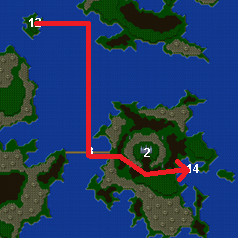
\includegraphics[scale=0.7]{../Graphics/Maps/11. To Zezat's Fleet.png}
\end{misc}

\switchcolumn*
\vspace{-5.685cm}
\begin{enumerate}[resume]
    \item Head below deck and enter the room on the right
\end{enumerate}

\begin{boss}{Gabbledeak}
	\varwb
    \begin{notes}
        \item \bossHl{Kunai is the right weapon}
    \end{notes}
	\begin{round}{1}
		\faris Item \then \unequip{\kunai} \then Put near the bottom \then \battleGroup{Defend}
        \galuf Defend
        \bartz \leftCommand{\gilToss}
	\end{round}
	\varwe
\end{boss}

\switchcolumn
\begin{misc}{Menu Here}
    \insertScreenshot{../Graphics/Misc/16. Gilgamesh 3 Menu.png}
\end{misc}

\switchcolumn
\begin{menu}{Before Interacting with Gilgamesh}
    \varwb
    \begin{itemMenu}
        \hiPotionMenu \ally{Anyone low on HP}
    \end{itemMenu}
    \begin{jobMenu}
        \bartz Chemist \textbf{(\pointUp)(\pointRight)} \ability{!\gilToss} \optimize
        \galuf Time Mage \textbf{(2\pointLeft)(\pointUp)}
    \end{jobMenu}
    \varwe
\end{menu}

\begin{boss}{Gilgamesh}
	\varwb
	\begin{round}{1}
		\faris \hiPotion \space \then \ally{Faris}
        \bartz Defend
        \lenna \leftCommand{\release}
        \item \bossMenu{Group Combine items together}
        \item \bossMenu{\textbf{Revivify} \mbox{\switch}\textbf{Maiden's Kiss}}
        \item \bossMenu{\textbf{Antidote} \mbox{\switch}\textbf{Phoenix Down}}
        \item \bossMenu{\textbf{Eyedrop}}
        \vspace{1mm}
        \item[] \insertBattleMenu{../Graphics/Battle/9. Gilgamesh 2 Menu.png}
	\end{round}
    \begin{bossPart}{If Death Misses}
        \galuf \leftCommand{\dimenAbility} \then \reset
    \end{bossPart}
	\varwe
\end{boss}

\begin{menu}{After Gilgamesh}
    \varwb
    \begin{jobMenu}
        \galuf Thief \textbf{(2\pointRight)} \ability{!\escape}
    \end{jobMenu}
    \varwe
\end{menu}

\begin{enumerate}[resume]
    \item Head below deck and enter the room on the left
\end{enumerate}

\end{paracol}
\chapter{Barrier Tower}

\vspace{\baselineskip}

\begin{paracol}{2}

\begin{enumerate}
    \item Start heading up the tower
    \item Grab the \pickup{9000 Gil} chest on the 2nd floor
    \item Grab the \pickup{18000 Gil} chest on the 6th floor
    \item Take the right stairwell on the 9th floor
\end{enumerate}

\begin{boss}{Atomos}
	\varwb
	\begin{bossPart}{Part 1}
		\galufLenna[\bossHl{(Rest)}] Defend
        \bartz \leftCommand{\drink} \then \heroDrink
        \bartz \leftCommand{\drink} \then \speedDrink
        \bartz \leftCommand{\drink} \then \heroDrink
        \bartz \leftCommand{\drink} \then \heroDrink
	\end{bossPart}
    \begin{bossPart}{Part 2}
        \bartz[\bossHl{(4x)}] \rightCommand{\gilToss}
        \item \bossMenu{Previous menuing if needed}
        \vspace{1mm}
        \item[] \insertBattleMenu{../Graphics/Battle/9. Gilgamesh 2 Menu.png}
	\end{bossPart}
	\varwe
\end{boss}

\begin{enumerate}[resume]
    \item Enter the submarine, return, wait for Galuf to finish grieving
    \item Head to Guido's Cave
\end{enumerate}

\begin{misc}{Path to Guido's Cave}
    \begin{itemize}
        \item East until you hit a set of rocks
        \item North until you see rocks on the far left side of the screen
        \item West until you hit rocks
        \item North until you see the cave
    \end{itemize}
\end{misc}

\begin{menu}{After Arriving at Guido's Cave}
    \varwb
    \begin{jobMenu}
        \bartz Ninja \textbf{(\pointLeft)(\pointDown)(\pointLeft)} \ability{!\escape} \optimize
    \end{jobMenu}
    \varwe
\end{menu}

\begin{encounter}{Radiator x2 (400 EXP)}
	\varwb
	\begin{notes}
		\item \encounterHl{Don't flee buffer}
	\end{notes}
	\begin{round}{1}
		\bartz \leftCommand{\throw} \then \flameScroll
	\end{round}
	\varwe
\end{encounter}

\begin{enumerate}[resume]
    \item Chest order is: middle \then top left \then \battleGroup{enter the new room} \then top left \then bottom left
\end{enumerate}

\switchcolumnTwice[*]
\begin{encounter}{Radiator x4 (1066 EXP)}
	\varwb
	\begin{notes}
		\item \encounterHl{Don't flee buffer}
	\end{notes}
	\begin{round}{1}
		\bartz \leftCommand{\throw} \then \flameScroll
	\end{round}
	\varwe
\end{encounter}

\switchcolumn
\begin{steproute}{Radiator x4 Backup}
    If you can't find a Radiator x4 encounter (rare) there is a backup outside Moore
\end{steproute}

\switchcolumn
\begin{menu}{After Reaching the End}
    \varwb
    \begin{jobMenu}
        \lenna Time Mage \textbf{(2\pointLeft)(\pointUp)}
    \end{jobMenu}
    \begin{magicMenu}
        \lenna \exit
    \end{magicMenu}
    \varwe
\end{menu}

\end{paracol}
\newpage
\chapter{Forest of Moore}

\vspace{\baselineskip}

\begin{paracol}{2}

\begin{enumerate}
    \item Head to the Forest of Moore
\end{enumerate}

\begin{misc}{Path to the Forest of Moore}
    \begin{itemize}
        \item West until you hit a wall
        \item Follow the walls around the northwest out of the trench
        \item Go straight west and count corals on the top edge of the screen
        \item After the third coral, go south
        \item Once you can, go east and north to the emerge point
    \end{itemize}
\end{misc}

\switchcolumn
\begin{steproute}{En Route to the Forest of Moore}
    \insertStep{../Graphics/Steps/142. Guido's Cave 4.jpg}
    \insertStep{../Graphics/Steps/143. Forest of Moore 1.jpg}
\end{steproute}

\switchcolumn
\newpage
\begin{misc}{First Screen Directions}
    \begin{itemize}
        \item Up until the chest and then mostly right
    \end{itemize}
\end{misc}

\begin{enumerate}[resume]
    \item Grab the \pickup{2500 Gil} chest directly north after entering
\end{enumerate}

\switchcolumn
\begin{steproute}{After the 2500 Gil Chest}
    \insertStep{../Graphics/Steps/144. Forest of Moore Enc 1.jpg}
    \insertStep{../Graphics/Steps/145. Forest of More 2.jpg}
    \insertStep{../Graphics/Steps/146. Forest of More 3.jpg}
\end{steproute}

\switchcolumn*
\begin{misc}{Second Screen Directions}
    \begin{itemize}
        \item Right until the first encounter
        \item Up until the second encounter 
        \item Right immediately afterward and grab the chest to the right of the tree
    \end{itemize}
\end{misc}

\switchcolumn
\begin{steproute}{Before the 9500 Gil Chest}
    \insertStep{../Graphics/Steps/147. Forest of Moore Enc 2.jpg}
    \insertStep{../Graphics/Steps/148. Forest of Moore Enc 3.jpg}
\end{steproute}

\switchcolumn
\begin{enumerate}[resume]
    \item Grab the \pickup{9500 Gil} chest on the east side before heading back west to the third screen
\end{enumerate}

\switchcolumn
\begin{steproute}{After the 9500 Gil Chest}
    \insertStep{../Graphics/Steps/149. Forest of Moore Enc 4.jpg}
\end{steproute}

\switchcolumn*
\begin{misc}{Third Screen Directions}
    \begin{itemize}
        \item Mostly up until the encounter
        \item Up until you hit a tree and then keep right until the chest at the top
    \end{itemize}
\end{misc}

\switchcolumn
\begin{steproute}{Before the Morning Star}
    \insertStep{../Graphics/Steps/150. Forest of Moore Enc 5.jpg}
\end{steproute}

\switchcolumn
\begin{enumerate}[resume]
    \item Grab the \pickup{Morning Star} chest at the top of the screen before the fire cutscene
\end{enumerate}

\switchcolumn
\begin{steproute}{Fire Cutscene}
    \insertStep{../Graphics/Steps/151. Forest of Moore 3.jpg}
    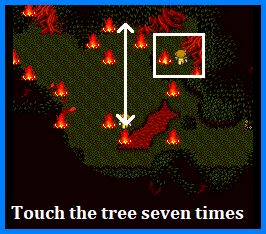
\includegraphics[scale=0.449]{../Graphics/Steps/152. Forest of Moore 4.jpg}
    \insertStep{../Graphics/Steps/153. Forest of Moore 5.jpg}
\end{steproute}

\switchcolumn*
\begin{enumerate}[resume]
    \item After the fire cutscene, heal with the lake
    \item After emerging, grab the \pickup{Flame Shield} chest to the right
    \item Go down and bit and head left (below the tree)
    \item Head up once you see the chest
\end{enumerate}

\switchcolumn
\begin{steproute}{Before Seal Guardians}
    \insertStep{../Graphics/Steps/154. Forest of Moore Enc 6.jpg}
    \insertStep{../Graphics/Steps/155. Forest of Moore Enc 7.jpg}
    \insertStep{../Graphics/Steps/156. Forest of More Enc 8.jpg}
    \insertStep{../Graphics/Steps/157. Forest of Moore Enc 9.jpg}
\end{steproute}

\switchcolumn
\begin{menu}{Before Seal Guardians}
    \varwb
    \begin{jobMenu}
        \lenna Samurai \textbf{(\pointLeft)(\pointDown)} \optimize
        \bartz Chemist \textbf{(\pointUp)(\pointRight)} \ability{!\gilToss} \optimize
        \faris Samurai \textbf{(\pointLeft)(\pointDown)} \equip{\goldShield}
        \galuf Samurai \textbf{(\pointLeft)(\pointDown)} \optimize
    \end{jobMenu}
    \begin{itemMenu}
        \hiPotionMenu \ally{Anyone not near full HP}
    \end{itemMenu}
    \varwe
\end{menu}

\begin{boss}{Seal Guardians}
    \varwb
    \begin{round}{1}
        \bartz \rightCommand{\gilToss}
        \everyoneElse \leftCommand{\gilToss}
    \end{round}
    \varwe
\end{boss}

\begin{boss}{Exdeath}
    \varwb
    \begin{round}{1}
        \galuf Item \then \phoenixDown \space \then \ally{Galuf}
    \end{round}
    \varwe
\end{boss}

\end{paracol}
\chapter{Exdeath's Castle}

\vspace{\baselineskip}

\begin{paracol}{2}

\begin{enumerate}
    \item Head to Exdeath's Castle
\end{enumerate}

\switchcolumn
\begin{misc}{Path to Exdeath's Castle}
    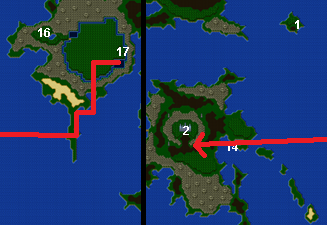
\includegraphics[scale=0.7]{../Graphics/Maps/12. To Exdeath's Castle.png}
\end{misc}

\switchcolumnTwice[*]
\begin{steproute}{Before Entering the Castle}
    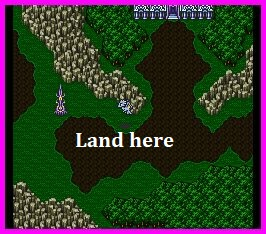
\includegraphics[scale=0.452]{../Graphics/Steps/158. Exdeath's Castle 1.jpg}
    \insertStep{../Graphics/Steps/159. Exdeath's Castle 2.jpg}
\end{steproute}

\switchcolumn
\begin{menu}{After the Half Step}
    \varwb
    \begin{jobMenu}
        \cara Ninja \textbf{(\pointLeft)(\pointDown)(\pointLeft)} \ability{\dash}
        \faris Mediator \textbf{(\pointUp)}       
    \end{jobMenu}
    \varwe
\end{menu}

\switchcolumnTwice[*]
\begin{enumerate}[resume]
    \item On the 2nd screen post transformation, activate the top left lever to grab the \pickup{Ice Shield}
\end{enumerate}

\switchcolumn
\begin{steproute}{MagicDragon}
    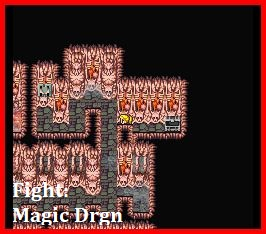
\includegraphics[scale=0.452]{../Graphics/Steps/160. Exdeath's Castle Enc 1.jpg}
\end{steproute}

\switchcolumn
\begin{encounter}{MagicDragon}
	\varwb
	\begin{notes}
		\item \encounterHl{Don't flee buffer}
	\end{notes}
	\begin{round}{1}
		\cara \leftCommand{\throw} \then \thunderScroll
        \bartz \rightCommand{\gilToss}
        \item \encounterHl{Be careful Lenna doesn't get her turn here}
        \faris \leftCommand{\catch}
	\end{round}
	\varwe
\end{encounter}

\switchcolumn
\begin{misc}{Menu Here}
    \insertScreenshot{../Graphics/Misc/17. Exdeath's Castle Menu.png}
\end{misc}

\switchcolumn
\begin{menu}{Before the Next Encounter}
    \varwb
    \begin{jobMenu}
        \faris Blue Mage \textbf{(\pointDown)(\pointLeft)(\pointDown)} \ability{!\gilToss}
        \begin{itemize}
            \item[] \equip{\iceShield}
        \end{itemize}
        \bartz Ninja \textbf{(\pointLeft)(\pointDown)(\pointLeft)} \ability{!\gilToss}
        \begin{itemize}
            \item[] \equip{\boneMail}
        \end{itemize}
        \lenna Blue Mage \textbf{(\pointDown)(\pointLeft)(\pointDown)} \ability{!\control}
        \begin{itemize}
            \item[] \optimize
        \end{itemize}
        \cara Mediator \textbf{(\pointUp)} \ability{\learning}
        \begin{itemize}
            \item[] \optimize
        \end{itemize}
    \end{jobMenu}
    \begin{itemMenu}
        \hiPotionMenu \ally{People missing 100+ HP}
    \end{itemMenu}
    \varwe
\end{menu}

\switchcolumn*
\begin{steproute}{MagicDragon, DarkWizard, TwinLizard}
    \insertStep{../Graphics/Steps/161. Exdeath's Castle Enc 2.jpg}
\end{steproute}

\switchcolumn
\begin{encounter}{MagicDragon, DarkWizard, TwinLizard}
	\varwb
	\begin{notes}
		\item \encounterHl{Don't flee buffer}
		\item \encounterHl{Make sure someone is hit by L.2 Old}
	\end{notes}
	\begin{round}{1}
		\bartz \leftCommand{\throw} \then \thunderScroll
        \cara Defend
        \faris Defend
        \lenna \rightCommand{\control} \then \enemy{MagicDragon}
	\end{round}
    \begin{round}{2}
		\bartz Defend
        \cara Defend
        \faris Defend
        \lenna \ltwoOld
        \item \encounterHl{Make sure it hits before continuing}
	\end{round}
    \begin{round}{3}
		\bartz Wait for L.2 Old cast \then \rightCommand{\gilToss}
        \cara \leftCommand{\catch}
	\end{round}
	\varwe
\end{encounter}

\switchcolumnTwice[*]
\begin{menu}{After the Encounter}
    \varwb
    \begin{jobMenu}
        \lenna Knight \textbf{(A)}
        \bartz Chemist \textbf{(\pointUp)(\pointRight)} \ability{!\gilToss}
        \begin{itemize}
            \item[] \optimize \space \then \unequip{Weapon}
        \end{itemize}
        \cara Thief \textbf{(2\pointRight)} \ability{!\escape}
    \end{jobMenu}
    \varwe
\end{menu}

\switchcolumn
\begin{steproute}{Before the Ether Chest}
    \insertStep{../Graphics/Steps/162. Exdeath's Castle 3.jpg}
\end{steproute}

\switchcolumn
\begin{enumerate}[resume]
    \item Grab the \pickup{Ether} chest on the screen after the encounters
    \item \battleGroup{Escape is the right command}
\end{enumerate}

\switchcolumn
\begin{steproute}{Before Exdeath}
    \insertStep{../Graphics/Steps/163. Exdeath's Castle Enc 3.jpg}
    \insertStep{../Graphics/Steps/164. Exdeath's Castle 4.jpg}
    \insertStep{../Graphics/Steps/165. Exdeath's Castle 5.jpg}
    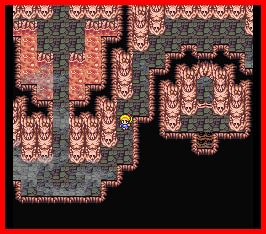
\includegraphics[scale=0.449]{../Graphics/Steps/166. Exdeath's Castle Enc 4.jpeg}
    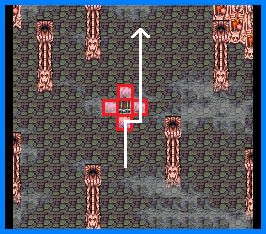
\includegraphics[scale=0.449]{../Graphics/Steps/167. Exdeath's Castle 6.jpeg}
    \insertStep{../Graphics/Steps/168. Exdeath's Castle 7.jpg}
\end{steproute}

\switchcolumn
\begin{menu}{Before Exdeath}
    \varwb
    \begin{jobMenu}
        \cara Blue Mage \textbf{(\pointDown)(\pointLeft)(\pointDown)} \ability{\dash} \optimize
    \end{jobMenu}
    \varwe
\end{menu}

\begin{boss}{Exdeath}
    \varwb
    \begin{round}{1}
        \cara \leftCommand{\blue} \then \ltwoOld
        \item \bossHl{Wait for 9 total "Can't run!!" messages}
        \item \bossNote{Have him selected and input when you see the 9th message disappear}
        \faris \leftCommand{\blue} \then \lfiveDeath
    \end{round}
    \varwe
\end{boss}

\end{paracol}
\chapter{World Three}

\vspace{\baselineskip}

\begin{paracol}{2}

\begin{enumerate}
    \item Head to Tycoon Castle
    \item Talk to Cara on the balcony
    \item Head southwest to Pirate's Cove
    \item Head to Guido's Cave (north past the castle \then follow the path until you hit Death Valley)
\end{enumerate}

\begin{boss}{Antlion}
    \varwb
    \begin{round}{1}
        \cara \leftCommand{\blue} \then \ltwoOld
        \bartz Defend \textbf{or} \hiPotion
    \end{round}
    \begin{round}{1}
        \cara \leftCommand{\blue} \then \lfiveDeath
    \end{round}
    \varwe
\end{boss}

\switchcolumnTwice[*]
\begin{enumerate}[resume]
    \item Dismount Boko before entering Guido's Cave
\end{enumerate}

\switchcolumn
\begin{misc}{Dismount Boko}
    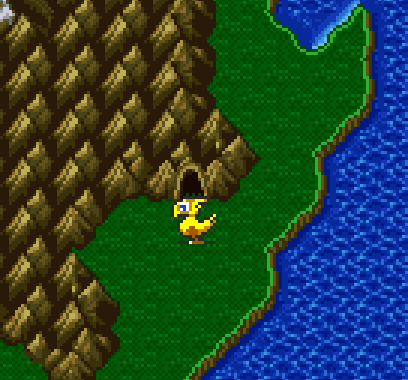
\includegraphics[scale=0.392]{../Graphics/Misc/18. Chocobo Discount.png}
\end{misc}

\switchcolumn*
\begin{enumerate}[resume]
    \item Head to the Pyramid of Moore
\end{enumerate}

\switchcolumn
\begin{steproute}{Before the Elder Tree}
    \insertStep{../Graphics/Steps/169. World 3 1.jpg}
\end{steproute}

\switchcolumn*
\begin{enumerate}[resume]
    \item Avoid this tile at the Elder Tree
\end{enumerate}

\switchcolumn
\begin{misc}{Elder Tree Cutscene Tile}
    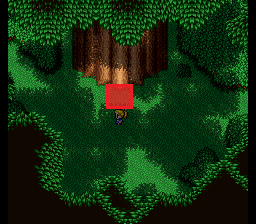
\includegraphics[scale=0.626]{../Graphics/Misc/19. Elder Tree Cutscene Tile.png}
\end{misc}

\switchcolumnTwice[*]
\begin{steproute}{Before the Pyramid}
    \insertStep{../Graphics/Steps/170. World 3 2.jpg}
    \insertStep{../Graphics/Steps/171. World 3 3.jpg}
\end{steproute}

\switchcolumn
\begin{menu}{Before Entering the Pyramid}
    \varwb
    \begin{jobMenu}
        \cara Samurai \textbf{(\pointLeft)(\pointDown)} \ability{\dash} \optimize
        \faris Ninja \textbf{(\pointLeft)(\pointDown)(\pointLeft) \ability{!\gilToss}}
    \end{jobMenu}
    \begin{itemMenu}
        \hiPotionMenu \ally{People missing 100+ HP}
    \end{itemMenu}
    \varwe
\end{menu}

\end{paracol}
\chapter{Pyramid of Moore}

\vspace{\baselineskip}

\begin{paracol}{2}

\begin{boss}{Gargoyles}
    \varwb
    \begin{round}{1}
        \faris \rightCommand{\gilToss}
        \cara \leftCommand{\gilToss}
        \bartz \rightCommand{\gilToss}
        \faris \rightCommand{\gilToss}
    \end{round}
    \varwe
\end{boss}

\begin{menu}{After Gargoyles}
    \varwb
    \begin{itemMenu}
        \hiPotionMenu \ally{People missing 100+ HP}
    \end{itemMenu}
    \begin{abilityMenu}
        \faris \ability{!\black}
    \end{abilityMenu}
    \begin{jobMenu}
        \cara Ninja \textbf{(\pointLeft)(\pointDown)(\pointLeft) \ability{!\white}}
        \bartz Thief \textbf{(2\pointRight)} \ability{!\combine} \optimize
        \begin{itemize}
            \item[] \equip{\stealthRobe, \greenBeret}
        \end{itemize}
    \end{jobMenu}
    \varwe
\end{menu}

\begin{enumerate}
    \item Keep track of how many Aspis encounters you get
\end{enumerate}

\switchcolumnTwice[*]
\begin{encounter}{Aspis}
    \varwb
    \begin{round}{1}
        \bartz \rightCommand{\combine} \then \battleGroup{\hiPotion \space + \phoenixDown} \textit{(RESURRECTION)} \then \enemy{Aspis} 
    \end{round}
    \varwe
\end{encounter}

\switchcolumn
\begin{steproute}{Aspis Adjustments}
    \insertStep{../Graphics/Steps/172. Pyramid (0 enc Snakes).jpg}
    \insertStep{../Graphics/Steps/173. Pyramid (2 encs Re-enter).jpg}
\end{steproute}

\switchcolumn
\begin{enumerate}[resume]
    \item Stop and wait for the spikes to come out to get poisoned
\end{enumerate}

\switchcolumn
\begin{misc}{If You Get a MachinHead}
    \begin{notes}
        \item \miscHl{Need to get Lamia's Kiss off before he gets a turn}
    \end{notes}
    \begin{round}{1}
        \bartz \rightCommand{\combine} \then \battleGroup{\maidensKiss \space + \eyedrop} \textit{(LAMIA'S KISS)} \then \enemy{MachinHead}
        \cara \leftCommand{\throw} \then \thunderScroll 
        \faris \leftCommand{\throw} \then \thunderScroll 
    \end{round}
    \begin{round}{2}
        \bartz \rightCommand{\combine} \then \battleGroup{\eyedrop \space + \revivify} \textit{(ELEMENTAL EDGE)} \then \enemy{MachinHead}
        \cara \leftCommand{\throw} \then \thunderScroll 
        \faris \leftCommand{\throw} \then \thunderScroll 
    \end{round}
\end{misc}

\switchcolumn
\begin{menu}{After Opening the Sarcophagus}
    \varwb
    \begin{jobMenu}
        \bartz Knight \textbf{(A)} \ability{!\black} \optimize
    \end{jobMenu}
    \begin{itemMenu}
        \hiPotionMenu \ally{Bartz}
    \end{itemMenu}
    \varwe
\end{menu}

\begin{boss}{Mummy x3}
    \varwb
    \begin{round}{1}
        \cara \leftCommand{\throw} \then \flameScroll
        \faris \leftCommand{\throw} \then \flameScroll
        \bartz \rightCommand{\black} \then \fire
    \end{round}
    \varwe
\end{boss}

\begin{menu}{After Mummies}
    \varwb
    \begin{jobMenu}
        \faris Mediator \textbf{(\pointUp)}
        \cara Thief \textbf{(2\pointRight)} \ability{!\escape}
    \end{jobMenu}
    \varwe
\end{menu}

\switchcolumn
\begin{steproute}{After Mummies}
    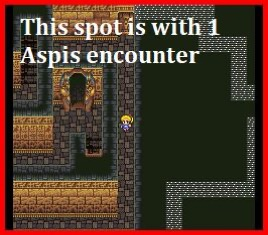
\includegraphics[scale=0.448]{../Graphics/Steps/174. Pyramid Enc 1.jpg}
    \insertStep{../Graphics/Steps/175. Pyramid 1.jpg}
\end{steproute}

\switchcolumn
\begin{enumerate}[resume]
    \item \battleGroup{Escape is the right command}
    \item Don't use the 2nd switch before the chest room
    \item Use the left switch to get the chests
    \item Grab the \pickup{9000 Gil} and \pickup{8000 Gil} chests on the right
\end{enumerate}

\switchcolumn*
\begin{steproute}{After the Two Chests}
    \insertStep{../Graphics/Steps/176. Pyramid Enc 2.jpg}
    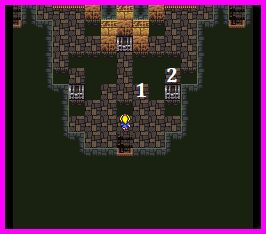
\includegraphics[scale=0.449]{../Graphics/Steps/177. Pyramid 2.jpeg}
    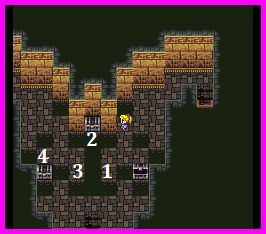
\includegraphics[scale=0.449]{../Graphics/Steps/178. Pyramid 3.jpeg}
\end{steproute}

\switchcolumn
\newpage
\begin{enumerate}[resume]
    \item Grab the \pickup{Gold Hairpin} chest on the right in the shifting floor room
    \item Take the right exit
    \item Grab the left chest containing \pickup{12000 Gil}
    \item Head back upstairs
    \item On the way out, grab the \pickup{Guard Ring} and \pickup{Ribbon}
\end{enumerate}

\switchcolumn
\begin{steproute}{After the Shifting Floor Room}
    \insertStep{../Graphics/Steps/179. Pyramid 4.jpg}
\end{steproute}

\end{paracol}
\chapter{Mirage}

\vspace{\baselineskip}

\begin{paracol}{2}

\begin{enumerate}
    \item Make your way back to the Elder Tree
\end{enumerate}

\switchcolumn
\begin{misc}{Menu Here}
    \insertScreenshot{../Graphics/Misc/20. Melusine Menu.png}
\end{misc}

\switchcolumn
\begin{menu}{Before Melusine}
    \varwb
    \begin{jobMenu}
        \cara Mediator \textbf{(\pointUp)} \ability{!\white}
    \end{jobMenu}
    \begin{magicMenu}
        \cara \cure \space \then \ally{Bartz (once)}
    \end{magicMenu}
    \varwe
\end{menu}

\begin{boss}{Melusine}
    \varwb
    \begin{round}{1}
        \cara \leftCommand{\release}
        \faris \leftCommand{\release}
        \bartz \rightCommand{\black} \then \fire
    \end{round}
    \varwe
\end{boss}

\switchcolumn*
\vspace{-1cm}
\begin{steproute}{After Melusine}
    \insertStep{../Graphics/Steps/180. Preamble 1.jpg}
\end{steproute}

\switchcolumn
\begin{menu}{On the World Map}
    \varwb
    \begin{itemMenu}
        \phoenixDownMenu \ally{Lenna}
        \antidoteMenu \ally{Everyone}
    \end{itemMenu}
    \begin{jobMenu}
        \cara Thief \textbf{(2\pointRight)} \ability{!\escape}
        \lenna Time Mage \textbf{(2\pointLeft)(\pointUp)}
        \bartz Freelancer \textbf{(\pointLeft)} \ability{!\escape \space !\combine}
    \end{jobMenu}
    \varwe
\end{menu}

\switchcolumn
\begin{steproute}{Before the Airship}
    \insertStep{../Graphics/Steps/181. Preamble 2.jpg}
\end{steproute}

\switchcolumn
\newpage
\begin{enumerate}[resume]
    \item Fly north to Mirage
\end{enumerate}

\switchcolumn
\begin{steproute}{Before Mirage}
    \insertStep{../Graphics/Steps/182. Preamble 3.jpg}
    \insertStep{../Graphics/Steps/183. Preamble 4.jpg}
\end{steproute}

\switchcolumn
\resume
\begin{enumerate}[resume]
    \item Head to the Inn
\end{enumerate}

\begin{shop}{Mirage Inn}
    \varwb
    \begin{itemize}
        \item \textit{Bottom NPC}
    \end{itemize}
    \begin{sell}
        \item \shopHl{All Armor and Weapons Except}
        \item \kunai
        \item \knife
        \item \ribbon
        \item \boneMail
    \end{sell}
    \begin{buy}
        \item \shopHl{(8)} \heroDrink \space \shopHl{(x11)}
        \item \shopHl{(6)} \speedDrink \space \shopHl{(x1)}
        \item \shopHl{(3)} \revivify \space \shopHl{(x31)}
    \end{buy}
    \begin{itemize}
        \item \textit{Top NPC}
    \end{itemize}
    \begin{buy}
        \item \shopHl{(3)} \phoenixDown \space \shopHl{(x2)}
        \item \shopHl{(4)} \maidensKiss \space \shopHl{(x11)}
        \item \shopHl{(5)} \antidote \space \shopHl{(x21)}
    \end{buy}
    \varwe
\end{shop}

\begin{enumerate}[resume]
    \item Head to the Magic Shop
\end{enumerate}

\begin{shop}{Mirage Magic Shop}
    \varwb
    \begin{buy}
        \item \shopHl{(1)} \size
        \item \shopHl{(4)} \float
    \end{buy}
    \varwe
\end{shop}

\begin{enumerate}[resume]
    \item Head to the Armory
    \item Interact with the back part of the desk to open the passage
\end{enumerate}

\begin{shop}{Mirage Hidden Armory}
    \varwb
    \begin{buy}
        \item \shopHl{(1)} \runningShoes \space \shopHl{(x1)}
    \end{buy}
    \varwe
\end{shop}

\switchcolumnTwice[*]
\begin{shop}{Mirage Armory}
    \varwb
    \begin{buy}
        \item \shopHl{(1)} \crystalShield \space \shopHl{(x1)}
    \end{buy}
    \varwe
\end{shop}

\switchcolumn
\begin{steproute}{Leaving Mirage}
    \insertStep{../Graphics/Steps/184. Preamble 5.jpg}
\end{steproute}

\switchcolumn
\begin{enumerate}[resume]
    \item Head north to The Void (where Tycoon used to be)
\end{enumerate}
    
\end{paracol}
\newpage
\chapter{Interdimensional Rift}

\vspace{\baselineskip}

\begin{paracol}{2}

\begin{enumerate}
    \item \battleGroup{Escape is the right command}
    \item Make your way through the Desert
\end{enumerate}

\switchcolumn
\begin{steproute}{Desert}
    \insertStep{../Graphics/Steps/185. Desert Enc 1.jpg}
    \insertStep{../Graphics/Steps/186. Desert Enc 2.jpg}
    \insertStep{../Graphics/Steps/187. Desert 1.jpg}
    \insertStep{../Graphics/Steps/188. Desert 2.jpg}
    \insertStep{../Graphics/Steps/189. Desert Enc 3.jpg}
\end{steproute}

\switchcolumn*
\begin{enumerate}[resume]
    \item Make your way through Mirage
    \item Make your way through the Forest
\end{enumerate}

\switchcolumn
\begin{steproute}{Leaving Mirage}
    \insertStep{../Graphics/Steps/190. Forest 1 (Re-enter).jpg}
\end{steproute}

\switchcolumn
\begin{misc}{Path Through the Forest}
    \begin{itemize}
        \item Right and up
        \item Left around the tree
        \item Up+right to the chest
    \end{itemize}
\end{misc}

\begin{enumerate}[resume]
    \item Grab the \pickup{Dragon Fang} chest at the top of the first screen
\end{enumerate}

\begin{misc}{Path Through the Forest}
    \begin{itemize}
        \item Stick to the bottom edge as you go right
        \item Right until you hit a tree
        \item Down until you are horizontal to the left chest
        \item Right until you see a chest below
    \end{itemize}
\end{misc}

\switchcolumn
\begin{steproute}{Forest}
    \insertStep{../Graphics/Steps/191. Forest Enc 1.jpg}
    \insertStep{../Graphics/Steps/192. Forest Enc 2.jpg}
\end{steproute}

\switchcolumn*
\begin{enumerate}[resume]
    \item Grab the \pickup{Ribbon} chest at the base of the tree
\end{enumerate}

\begin{misc}{Path Through the Forest}
    \begin{itemize}
        \item Down to Calofisteri
    \end{itemize}
\end{misc}

\begin{menu}{Before Calofisteri}
    \varwb
    \begin{jobMenu}
        \faris Blue Mage \textbf{(\pointDown)(\pointLeft)(\pointDown)} \equip{\runningShoes}
        \cara Blue Mage \textbf{(\pointDown)(\pointLeft)(\pointDown)}
    \end{jobMenu}
    \varwe
\end{menu}

\begin{boss}{Calofisteri}
    \varwb
    \begin{round}{1}
        \item Wait for her attack
        \item Queue L.2 Old during her attack animation
    \end{round}
    \begin{round}{2}
        \faris \leftCommand{\blue} \then \ltwoOld
        \item \bossHl{Wait for 17 total "Can't run!!" messages}
        \item \bossNote{Have her selected and input when you see the 17th message disappear}
        \cara \leftCommand{\blue} \then \lfiveDeath
    \end{round}
    \begin{bossPart}{If Reflect or Cara Dies}
        \lenna \leftCommand{\dimenAbility} \then \reset
    \end{bossPart}
    \varwe
\end{boss}

\switchcolumnTwice[*]
\begin{menu}{After Calofisteri}
    \varwb
    \begin{jobMenu}
        \cara White Mage \textbf{(2\pointRight)(\pointDown)}
        \lenna Knight \textbf{(A)} \ability{!\dimenAbility} \optimize
    \end{jobMenu}
    \begin{magicMenu}
        \lenna \float \space \then \ally{Cara}
        \cara \size \space \then \ally{Lenna}
        \cara \life \space \then \ally{Anyone dead}
    \end{magicMenu}
    \begin{equipMenu}
        \faris \unequip{All}
        \bartz \optimize
    \end{equipMenu}
    \begin{jobMenu}
        \faris Chemist \textbf{(\pointUp)(\pointRight)} \ability{!\gilToss}
        \cara Thief \textbf{(2\pointRight)}
    \end{jobMenu}
    \varwe
\end{menu}

\switchcolumn
\begin{steproute}{Cavern}
    \insertStep{../Graphics/Steps/193. Forest 2.jpg}
    \insertStep{../Graphics/Steps/194. Cavern Enc 1.jpg}
    \insertStep{../Graphics/Steps/195. Cavern 1 (Re-enter).jpg}
    \insertStep{../Graphics/Steps/196. Cavern 2 (Re-enter).jpg}
\end{steproute}

\switchcolumn
\begin{enumerate}[resume]
    \item \battleGroup{Escape is the left command}
    \item Hold B when transitioning out of the save room and dodge Omega around the bottom
\end{enumerate}

\switchcolumn
\begin{steproute}{Before Apanda}
    \insertStep{../Graphics/Steps/197. Cavern 3.jpg}
\end{steproute}

\switchcolumn
\begin{menu}{Before Opening the Book}
    \varwb
    \begin{jobMenu}
        \cara Samurai \textbf{(\pointLeft)(\pointDown)}
    \end{jobMenu}
    \begin{rowMenu}
        \caraFarisBartz Frontrow
        \swap Cara \switch Faris
    \end{rowMenu}
    \varwe
\end{menu}

\begin{boss}{Apanda}
    \varwb
    \begin{bossPart}{Part 1}
        \bartz[\bossHl{(1x)}] \rightCommand{\combine} \then \battleGroup{\revivify \space + \antidote} \textit{(SAMSON POWER)} \then \ally{Faris}
        \faris[\bossHl{(1x)}] \leftCommand{\drink} \then \speedDrink
        \cara[\bossHl{(Rest)}] Defend
        \lenna[\bossHl{(Rest)}] \leftCommand{\guard}
    \end{bossPart}
    \begin{bossPart}{Part 2}
        \bartz[\bossHl{(1x)}] \rightCommand{\combine} \then \battleGroup{\revivify \space + \maidensKiss} \textit{(KISS OF BLESSING)} \then \enemy{Apanda}
    \end{bossPart}
    \begin{bossPart}{Part 3}
        \faris[\bossHl{(2x)}] \leftCommand{\drink} \then \heroDrink
        \bartz[\bossHl{(2x)}] \rightCommand{\combine} \then \battleGroup{\revivify \space + \antidote} \textit{(SAMSON POWER)} \then \ally{Faris}
    \end{bossPart}
    \begin{bossPart}{Part 4}
        \faris[\bossHl{(3x)}] \rightCommand{\gilToss}
        \bartz[\bossHl{(Rest)}] Defend
    \end{bossPart}
    \varwe
\end{boss}

\switchcolumnTwice[*]
\begin{menu}{After Apanda}
    \varwb
    \begin{jobMenu}
        \cara Thief \textbf{(2\pointRight)} \ability{!\gilToss}
    \end{jobMenu}
    \varwe
\end{menu}

\newpage
\begin{enumerate}[resume]
    \item \battleGroup{Escape is the left command}
    \item Make your way through the Sky Pillars
\end{enumerate}

\switchcolumn
\vspace{-1cm}
\begin{steproute}{Sky Pillars}
    \insertStep{../Graphics/Steps/198. Floating Castle Enc 1.jpg}
    \insertStep{../Graphics/Steps/199. Floating Castle Enc 2.jpg}
    \insertStep{../Graphics/Steps/200. Floating Castle Enc 3.jpg}
\end{steproute}

\end{paracol}
\chapter{Floating Castle}

\vspace{\baselineskip}

\begin{paracol}{2}

\begin{enumerate}
    \item Take the right path outside (bottom door) after entering the Castle
    \item Grab the \pickup{Running Shoes} chest and head to the castle basement
\end{enumerate}

\begin{menu}{Before Catastrophe}
    \varwb
    \begin{equipMenu}
        \faris \optimize
    \end{equipMenu}
    \varwe
\end{menu}

\begin{boss}{Catastrophe}
    \varwb
    \begin{bossPart}{Part 1}
        \bartz[\bossHl{(1x)}] \rightCommand{\combine} \then \battleGroup{\antidote \space + \turtleShell} \textit{(SPLIT SHELL)} \then \enemy{Catastrophe}
        \faris[\bossHl{(1x)}] \leftCommand{\drink} \then \heroDrink
    \end{bossPart}
    \begin{bossPart}{Part 2}
        \cara[\bossHl{(1x)}] \rightCommand{\gilToss}
        \bartz[\bossHl{(1x)}] \rightCommand{\combine} \then \battleGroup{\potion \space + \dragonFang} \textit{(DRAGON POWER)} \then \ally{Faris}
        \lenna[\bossHl{(1x)}] \rightCommand{\dimenAbility} \then \float \space \then \ally{Faris}
    \end{bossPart}
    \begin{bossPart}{Part 3}
        \faris[\bossHl{(3x)}] \rightCommand{\gilToss}
        \bartz[\bossHl{(2x)}] \rightCommand{\combine} \then \battleGroup{\revivify \space + \antidote} \textit{(SAMSON POWER)} \then \ally{Faris}
        \cara[\bossHl{(1x)}] \rightCommand{\gilToss}
        \lenna[\bossHl{(1x)}] Defend \textbf{or} \rightCommand{\dimenAbility} \then \float \space \then \ally{Faris}
    \end{bossPart}
    \varwe
\end{boss}

\begin{enumerate}[resume]
    \item \battleGroup{Escape is the left command}
    \item Head through the cell into the throne room
\end{enumerate}

\begin{boss}{Halicarnassus}
    \varwb
    \begin{notes}
        \item \bossNote{Faris can start Gil Tossing after being buffed twice}
    \end{notes}
    \begin{bossPart}{Part 1}
        \bartz[\bossHl{(3x)}] \rightCommand{\combine} \then \battleGroup{\revivify \space + \antidote} \textit{(SAMSON POWER)} \then \ally{Faris}
        \faris[\bossHl{(1x)}] \leftCommand{\drink} \then \heroDrink
        \cara[\bossHl{(1x)}] Defend
        \lenna[\bossHl{(Rest)}] \leftCommand{\guard}
        \faris[\bossHl{(2x)}] \rightCommand{\gilToss}
    \end{bossPart}
    \begin{bossPart}{Part 2}
        \cara[\bossHl{(1x)}] \rightCommand{\gilToss}
        \bartz Defend
        \faris[\bossHl{(1x)}] \rightCommand{\gilToss}
    \end{bossPart}
    \begin{bossPart}{Part 3}
        \cara Defend
        \bartz[\bossHl{(1x)}] \rightCommand{\combine} \then \battleGroup{\revivify \space + \antidote} \textit{(SAMSON POWER)} \then \ally{Faris}
        \faris[\bossHl{(1x)}] \rightCommand{\gilToss}
    \end{bossPart}
    \varwe
\end{boss}

\begin{enumerate}[resume]
    \item \battleGroup{Escape is the left command}
    \item Continue onward to the outside area
\end{enumerate}

\switchcolumn
\begin{misc}{Menu Here}
    \insertScreenshot{../Graphics/Misc/21. Twintania Menu.png}
\end{misc}

\switchcolumn
\begin{menu}{Before Twintania}
    \varwb
    \begin{itemMenu}
        \maidensKissMenu \ally{Everyone}
    \end{itemMenu}
    \begin{abilityMenu}
        \bartz \ability{!\hide \space in slot 1} \optimize
    \end{abilityMenu}
    \begin{jobMenu}
        \lenna Blue Mage \textbf{(\pointDown)(\pointLeft)(\pointDown)}
    \end{jobMenu}
    \varwe
\end{menu}

\begin{boss}{Twintania}
    \varwb
    \begin{bossPart}{Part 1}
        \bartz \leftCommand{\hide}
    \end{bossPart}
    \begin{bossPart}{Part 2}
        \item Wait until you cumulatively see 4 attacks or “Ineffective” prompts
        \bartz \leftCommand{\showAbility}
    \end{bossPart}
    \begin{bossPart}{Part 3}
        \bartz \rightCommand{\combine} \then \battleGroup{\hiPotion \space + \phoenixDown} \textit{(RESURRECTION)} \then \ally{Lenna} 
        \item \bossHl{Don't run buffer Lenna's attack}
        \item \bossNote{Wait for the text before queuing L.5 Death}
        \lenna \leftCommand{\blue} \then \lfiveDeath
    \end{bossPart}
    \varwe
\end{boss}

\begin{menu}{After Twintania}
    \varwb
    \begin{jobMenu}
        \lenna White Mage \textbf{(2\pointRight)(\pointDown)}
    \end{jobMenu}
    \begin{itemMenu}
        \elixirMenu \ally{Lenna}
    \end{itemMenu}
    \begin{magicMenu}
        \lenna \life \space \then \ally{Everyone}
    \end{magicMenu}
    \begin{jobMenu}
        \lenna Mystic Knight \textbf{(\pointRight)(\pointDown)} \optimize
        \faris Freelancer \textbf{(\pointLeft)} \equip{\ribbon \space in head slot}
    \end{jobMenu}
    \begin{abilityMenu}
        \bartz \ability{!\escape \space in slot 1} \optimize
    \end{abilityMenu}
    \varwe
\end{menu}

\end{paracol}
\chapter{The Void}

\vspace{\baselineskip}

\begin{paracol}{2}

\begin{enumerate}
    \item \battleGroup{Escape is the left command}
    \item Make your way towards Exdeath
\end{enumerate}

\begin{menu}{After the Cutscene}
	\varwb
    \begin{abilityMenu}
        \bartz \ability{!\gilToss} \optimize
        \lenna \ability{!\cover} 
        \begin{itemize}
            \item[] \equip{\knife, \crystalShield}
        \end{itemize}
    \end{abilityMenu}
    \begin{jobMenu}
        \faris Blue Mage \textbf{(\pointDown)(\pointLeft)(\pointDown)} \ability{\combine} 
        \begin{itemize}
            \item[] \equip{\runningShoes}
        \end{itemize} 
        \cara Monk \textbf{(\pointRight)} \ability{!\gilToss} \optimize
    \end{jobMenu}
    \begin{rowMenu}
        \swap Cara \switch Faris
        \swap Lenna \switch Bartz
    \end{rowMenu}
    \varwe
\end{menu}

\switchcolumn
\begin{misc}{Menu Here}
    \insertScreenshot{../Graphics/Misc/22. Exdeath Menu.png}
\end{misc}

\switchcolumn
\begin{boss}{Exdeath}
    \varwb
    \begin{bossPart}{Part 1 (Prep Lenna)}
        \bartz[\bossHl{(1x)}] \rightCommand{\combine} \then \battleGroup{\revivify \space + \space \maidensKiss} \textit{(KISS OF BLESSING)} \then \ally{Lenna}
        \faris[\bossHl{(1x)}] \rightCommand{\combine} \then \battleGroup{\eyedrop \space + \space \antidote{}} \textit{(RESTORATIVE)} \then \ally{Lenna}
        \cara[\bossHl{(1x)}] Defend
        \lenna[\bossHl{(1x)}] \leftCommand{\magicSword} \then \breakSpell
    \end{bossPart}
    \begin{bossPart}{Part 2 (Buff Cara)}
        \bartzFaris[\bossHl{(4x)}] \rightCommand{\combine} \then \battleGroup{\revivify \space + \space \antidote} \textit{(SAMSON POWER)} \then \ally{Cara}
        \lenna[\bossHl{(Rest)}] Defend
        \cara[\bossHl{(1x)}] Defend
        \bartzFaris[\bossHl{(4x)}] \rightCommand{\combine} \then \battleGroup{\revivify \space + \space \antidote} \textit{(SAMSON POWER)} \then \ally{Cara}
        \cara[\bossHl{(1x)}] \leftCommand{\kick}
    \end{bossPart}
    \begin{bossPart}{Part 3 (Buff Bartz)}
        \bartzFaris[\bossHl{(4x)}] \rightCommand{\combine} \then \battleGroup{\revivify \space + \space \antidote} \textit{(SAMSON POWER)} \then \ally{Bartz}
        \cara[\bossHl{(1x)}] \rightCommand{\gilToss}
        \bartzFaris[\bossHl{(2x)}] \rightCommand{\combine} \then \battleGroup{\revivify \space + \space \antidote} \textit{(SAMSON POWER)} \then \ally{Bartz}
    \end{bossPart}
    \begin{bossPart}{Part 4 (Prep Cara)}
        \bartz[\bossHl{(1x)}] \rightCommand{\combine} \then \battleGroup{\revivify \space + \space \maidensKiss} \textit{(KISS OF BLESSING)} \then \ally{Cara}
        \faris[\bossHl{(1x)}] \rightCommand{\combine} \then \battleGroup{\eyedrop \space + \space \antidote{}} \textit{(RESTORATIVE)} \then \ally{Cara}
        \item \bossNote{Let Exdeath get a turn here}
    \end{bossPart}
    \begin{bossPart}{Part 5}
        \bartz[\bossHl{(1x)}] \leftCommand{\gilToss}
        \cara[\bossHl{(1x)}] \rightCommand{\gilToss}
        \faris[\bossHl{(1x)}] \rightCommand{\combine} \then \battleGroup{\revivify \space + \space \antidote} \textit{(SAMSON POWER)} \then \ally{Bartz}
    \end{bossPart}
    \begin{bossPart}{Part 6}
        \bartz[\bossHl{(1x)}] \leftCommand{\gilToss}
        \item \bossNote{Make sure Faris has full ATB}
        \cara[\bossHl{(1x)}] \rightCommand{\gilToss}
    \end{bossPart}
    \varwe
\end{boss}

\begin{boss}{Neo Exdeath}
    \varwb
    \begin{bossPart}{Part 1}
        \item \bossNote{Wait for him to appear before queuing L.2 Old}
        \faris[\bossHl{(1x)}] \leftCommand{\blue} \then \ltwoOld
        \lenna[\bossHl{(1x)}] Fight \then \enemy{the body (\pointDown)}
        \bartz[\bossHl{(1x)}] Defend
        \cara[\bossHl{(1x)}] \leftCommand{\kick}
    \end{bossPart}
    \begin{bossPart}{Part 2}
        \faris[\bossHl{(1x)}] Wait for his attack \then \leftCommand{\blue} \then \lfiveDeath[\newline]
        \lennaFaris[\bossHl{(Rest)}] Defend
        \begin{itemize}
            \item \bossNote{If Break missed Lenna needs to attack again}
        \end{itemize}
        \bartz[\bossHl{(1x)}] \leftCommand{\gilToss}
        \cara[\bossHl{(1x)}] \leftCommand{\kick}
    \end{bossPart}
    \begin{bossPart}{Part 3}
        \bartz[\bossHl{(3x)}] \leftCommand{\gilToss}
        \cara[\bossHl{(1x)}] Fight \then \enemy{the head}
        \cara[\bossHl{(1x)}] \rightCommand{\gilToss}
        \cara[\bossHl{(1x)}] Fight \then \enemy{the head}
    \end{bossPart}
    \varwe
\end{boss}

\end{paracol}

%----------end of document----------%
\end{document}
